\section{Вычислительный эксперимент} \label{sec:experiments}

\subsection{Постановка эксперимента}

    В данной работе проводится несколько экспериментов для проверки теоретических результатов, разработанных в предыдущих разделах. Цель этих экспериментов -- сравнить предсказания с реальными наблюдениями в условиях управляемой среды.
    
    Приведем формальную постановку конкретной задачи для демонстрации процесса многократного обучения. Следуя постановке задачи \eqref{system}, пусть $\textbf{F}$ \eqref{R} -- пространство функций плотности вероятности. На шаге $t = 0$ берется начальное значение $f_0 \in \textbf{F}$ и выборка исходного множества $(\textbf{X}, \mathbf{y})$ из $f_0$ и принимаем $\epsilon$ за нормально распределенный шум. В данной работе рассматривается задача регрессии с функцией потерь $L$, то есть находится $\theta^*$ такая, что

    \begin{equation*} \label{regression}
        \theta^* = \text{argmin}_{\theta} L (\mathbf{y}, \textbf{X} \cdot \theta + \epsilon).
    \end{equation*} 

    Для того чтобы исследовать, как регуляризация, кросс-валидация и алгоритмы обучения влияют на теоретические результаты, используется линейная модель без регуляризации, обучаемая с помощью алгоритма стохастического градиентного спуска (SGD) с максимальным числом итераций $50$, модель гребневой регрессии (Ridge) без регуляризации, решаемая с помощью разложения Холески, и модель гребневой регрессии с кросс-валидацией (RidgeCV) с параметром регуляризации $0,1$, оптимизируемая с помощью сингулярного разложения (SVD). Модели и алгоритмы обучения реализованы в библиотеке Scikit-learn \citep{pedregosa2011scikit}.

    В данной работе используются синтетические исходные наборы данных, чтобы ограничить неизвестные сопутствующие факторы и изолировать эффект многократного обучения. В первом наборе данных входные данные $\textbf{X}$ нормально распределены, а $\mathbf{y}$ является линейной функцией $\textbf{X}$ с дополнительным нормальным шумом. В качестве второго набора данных берется задача Фридмана \citep{friedman1991multivariate}, которая не является линейной.
    Оба набора данных получены из библиотеки Scikit-learn \citep{pedregosa2011scikit} с помощью функций make\_regression() и make\_friedman1().
    Количество объектов в наборе данных $\textbf{X}$ равно $ N = 2000$, а количество признаков -- $10$.
    На шаге $t=0$ входные данные в обоих случаях являются н.о.р., связь между $\textbf{X}$ и $\mathbf{y}$ в первом случае линейная. Каждый эксперимент проводится десять раз, чтобы уменьшить влияние случайных факторов. 
    
    Для реализации среды моделирования используется пакет для воспроизведения экспериментов MLDev \citep{khritankov2021mldev}. Исходный код и данные для воспроизведения экспериментов можно найти в репозитории Gitlab \footnotemark.

    \footnotetext{Исходный код для экспериментов: \url{https://gitlab.com/repeated_ml/dynamic-systems-model}}

    В постановке эксперимента \emph{скользящее окно}, идентичная \citep{khritankov2023positive}, при раунде $r = 0$ сначала выбирается $30\%$ исходных данных $\textbf{X} \in \mathbb{R}^{N \times d}$, на которых обучается модель $h_0$ на $80\%$ подмножестве входных данных.   
    Затем, на каждом шаге $t$, случайным образом без замены выбирается элемент $(\mathbf{x}^i, y_i)$ -- признаки и целевую переменную элемента $i$ из оставшихся данных. Далее получается предсказание $y'_i$ из модели $y_i' = h_t(\mathbf{x^i})$ и сэмплируется $z_i \sim \mathcal{N}(y_i', s \cdot \sigma^2)$, где $s$ - \emph{приверженность} (adherehce,  \citep{khritankov2023positive}), параметр эксперимента, а $\sigma$ - средняя квадратичная ошибка предсказаний на удержанном $30\%$ подмножестве текущего набора с шагом $t - 1$. После этого удаляется самый ранний элемент из текущего набора и добавляется новый элемент $(\mathbf{x^i}, z_i)$ с вероятностью \emph{использование} (usage,  \citep{khritankov2023positive}) $p$ или элемент $(\mathbf{x^i}, y_i)$ с вероятностью $(1-p)$. Процедура повторяется до тех пор, пока не закончатся элементы исходного набора, то есть всего $0,7 \cdot N$ шагов. После каждых $T$ шагов $r$ увеличивается: $r = r + 1$ и модель машинного обучения $h_t$ обучается с размером обучения $80\%$ на активном множестве.

    В постановке \emph{обновлении выборки} модель $h_0$ обучается на всей выборке $\textbf{X}$ на раунде $r = 0$. Далее процедура очень похожа на обновление скользящего окна, но когда берется элемент $(\mathbf{x^i}, y_i)$ из активного множества, он заменяется, по тем же правилам, что и в постановке скользящее окно. Следствием такой модификации является то, что, во-первых, при обновлении выборки система будет автономной, так как процедура, а значит и оператор эволюции $\text{D}$, не зависят от шага $t$. Во-вторых, эксперимент с обновлением выборки можно проводить неограниченное количество шагов по времени, в то время как эксперимент со скользящим окном допускает не более $0,7 \cdot N$ итераций. 

    В обоих случаях размер активного множества остается постоянным -- $0,3 \cdot N$ для постановке скользящее окно и $N$ для обновления выборки. Действительно, в обоих постановках на каждом шаге удаляется и добавляется один элемент в активное множество. Отображение $\text{D}_t$ преобразует данные на каждом шаге $t$, поэтому для всех $t$ существует функция плотности данных $f_t$. Поскольку решается задача обучения с учителем, каждый шаг $T$ записываются невязки модели $h$ на отложенной выборке активного набора данных. Именно эти данные используются во всех экспериментах.

    Схемы обоих постановок эксперимента приведены на Рис.~\ref{ex_set}. 

    \begin{figure}[h!]
        \centering
        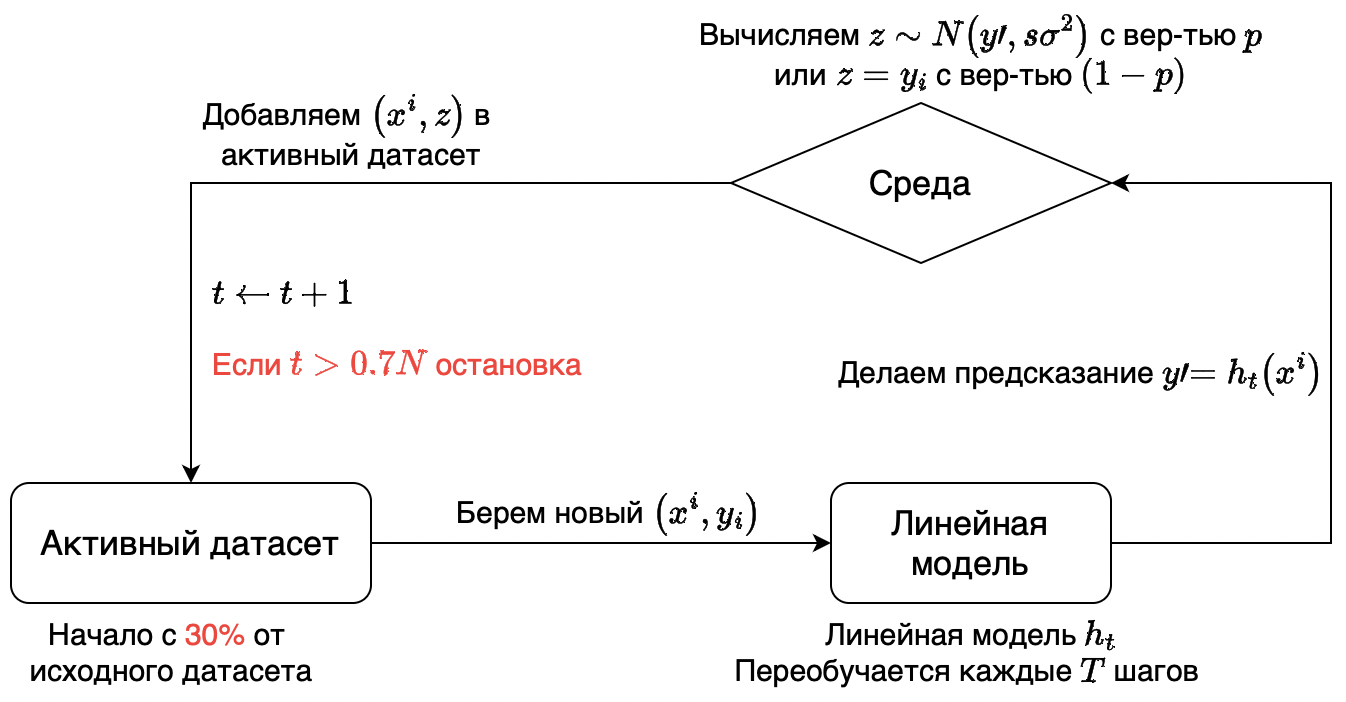
\includegraphics[width=0.49\linewidth]{pictures/Sliding window.png}
        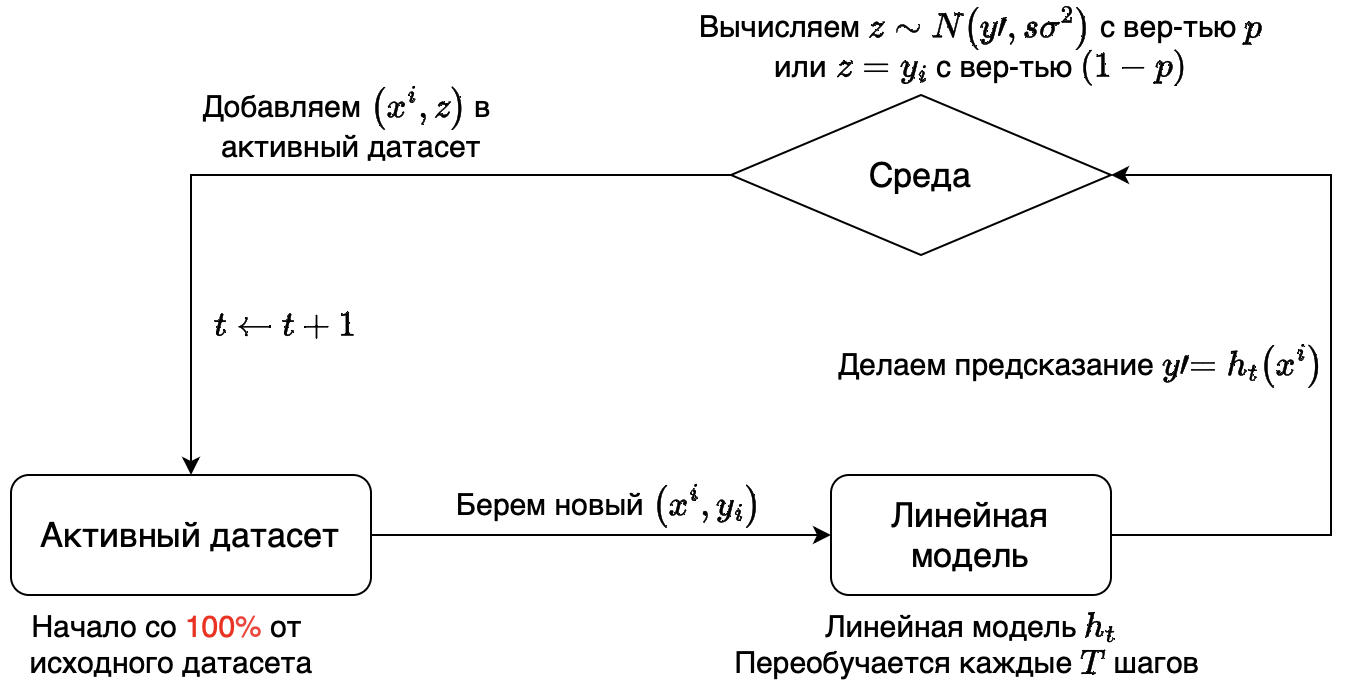
\includegraphics[width=0.49\linewidth]{pictures/Sampling update.png}
        
        \caption{Две различные постановки эксперимента. Скользящее окно (слева) и обновление выборки (справа). Красным цветом показаны различия двух систем.}
        \label{ex_set}
    \end{figure}

    Сбор данных занимает около двух часов для эксперимента в разделе~\ref{exp_1} и около часа для экспериментов в разделе~\ref{exp_2} и остальных. Все эксперименты проводились на ноутбуке с четырехъядерным процессором ARM-64 и воспроизводились на другом четырехъядерном настольном ПК без какого-либо аппаратного ускорения.

\subsection{Анализ ошибок прогнозирования} \label{exp_1}

    Согласно Теореме~\ref{delta} двумя возможными предельными распределениями $f_t$ являются дельта-функция $\delta(x)$ или нулевое распределение $\zeta(x)$. В этом эксперименте исследуется, как меняется стандартное отклонение ошибки предсказания с течением времени. Исходя из Леммы~\ref{moments} и Теоремы~\ref{delta}, в этом эксперименте должны наблюдаться два случая: стремление дисперсии к нулю (то есть стремление плотностей к дельта-функции) или стремление дисперсии к бесконечности (то есть стремление плотностей к нулевому распределению). По этой причине на каждые 10 шагов вычисляется стандартное отклонение разности $y_i - y_i'$. 

    Эксперимент проводится для различных значений использования $p$ -- какая часть предсказаний просматривается пользователями, вероятность включения $(\mathbf{x}^i, z_i)$ в текущий набор, и приверженностью $s$ -- насколько точно предсказания модели соблюдаются пользователями, параметр умножения $\sigma^2$ при выборке $z_i$. Также варьируется дисперсия нормального распределения шума $\epsilon$: $0.1, 0.3, 1, 3$ и $10$. На Рис.~\ref{3D} показан только результат с дисперсией шума $1$, для других значений картина аналогична. Другие рисунки можно найти в нашем репозитории. В этом эксперименте рассматривается модель регрессии SGD и синтетический линейный набор данных.

    \begin{figure}[h!]
        \centering
        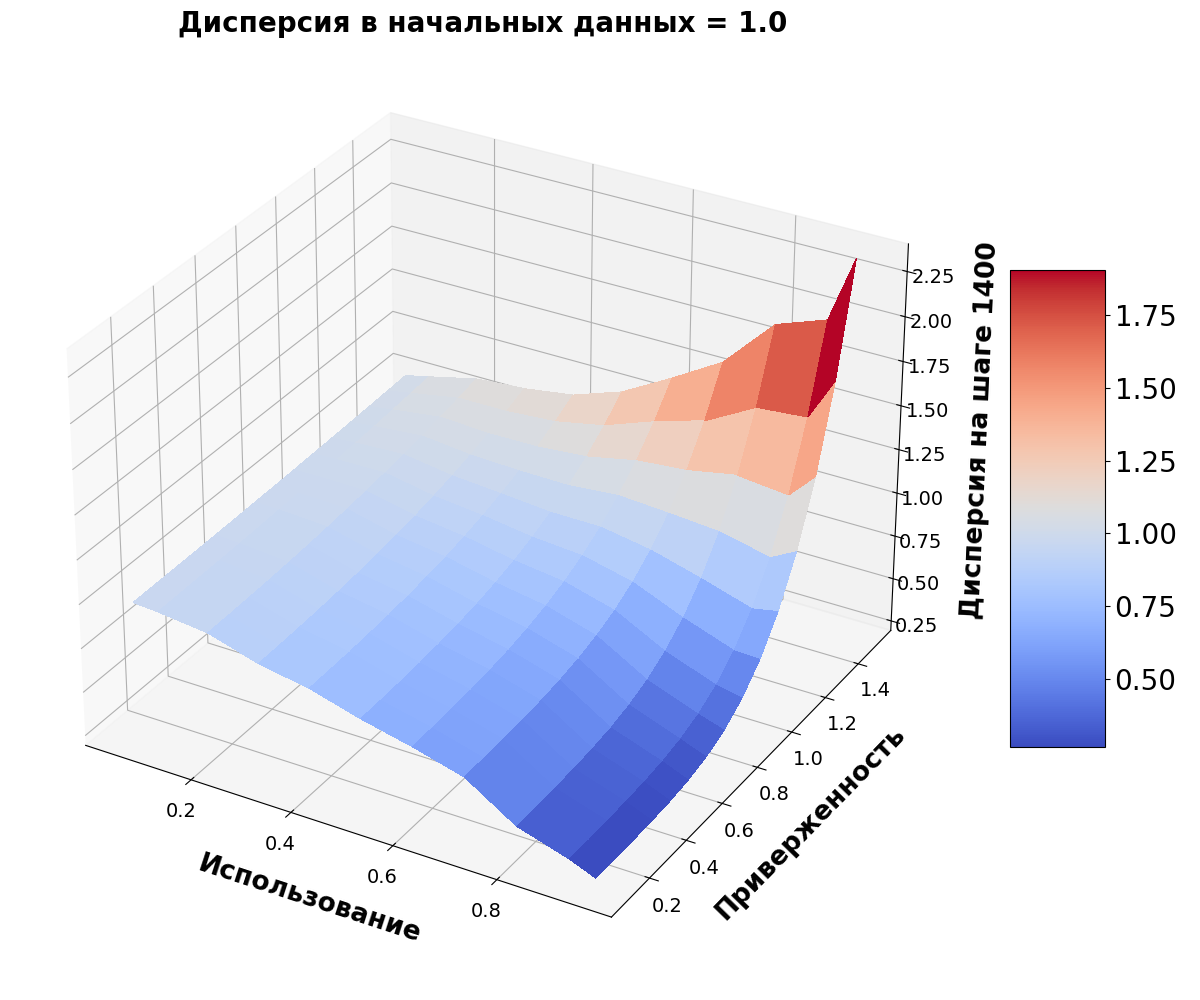
\includegraphics[width=0.49\linewidth]{pictures/3D_sw_1.0_synthetic_sgd_model_50.png}
        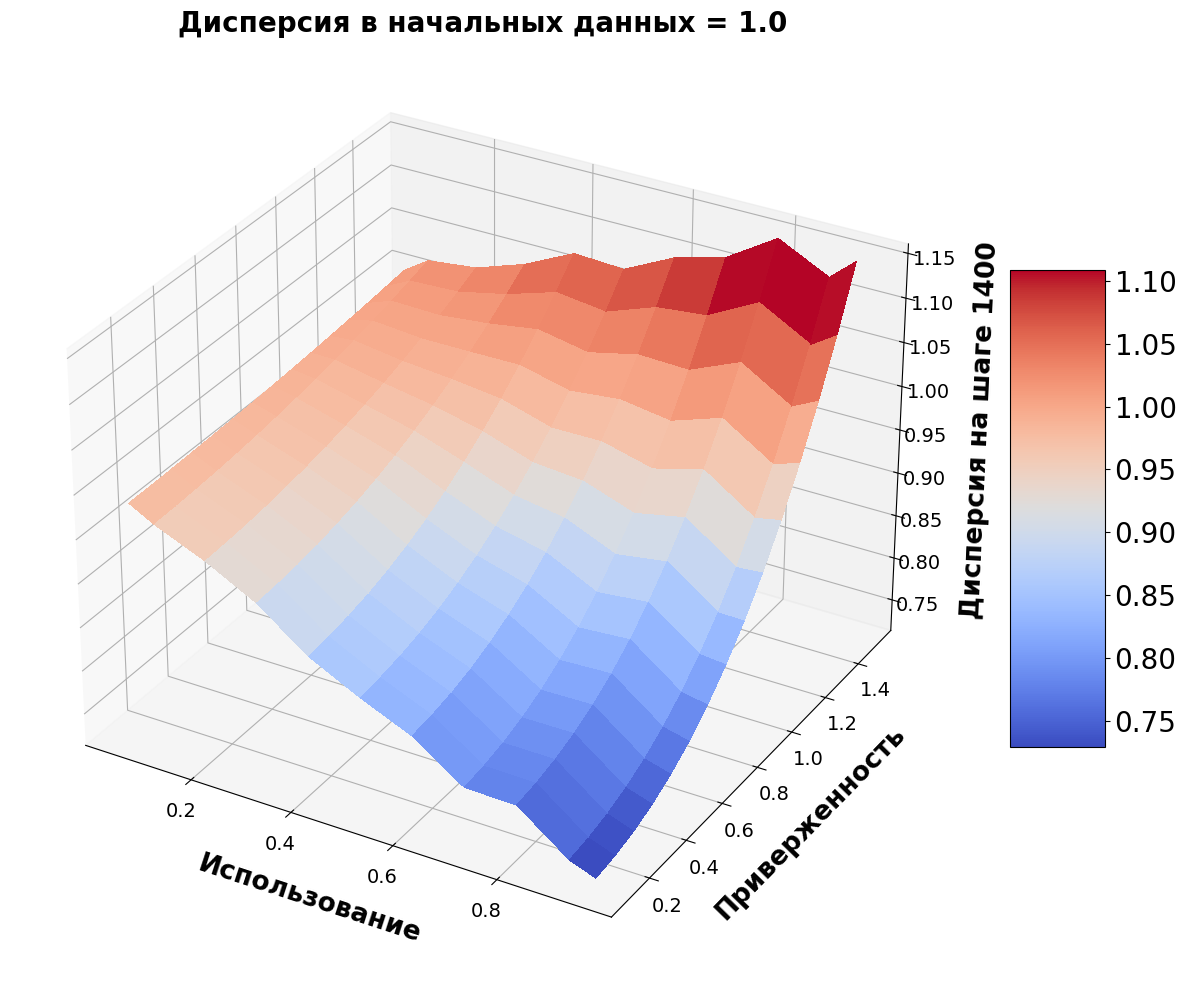
\includegraphics[width=0.49\linewidth]{pictures/3D_su_1.0_synthetic_sgd_model_50.png}
        
        \caption{Изменение стандартного отклонения ошибки модели для различных вариантов использования и приверженности. Скользящее окно (слева), обновление выборки (справа). График почти везде либо красный, либо синий, следовательно, Теорема~\ref{delta} применима на практике.}
        \label{3D}
    \end{figure}

    Как видно из Рис.~\ref{3D}, по мере увеличения использования $p$ и уменьшения приверженности $s$, отклонение уменьшается, так как в активный набор данных добавляется меньше зашумленных данных.

    Почти во всех случаях поверхность, показанная на Рис.~\ref{3D}, имеет красный или синий цвет, то есть для большинства комбинаций использования и приверженности наблюдается стремление либо к дельте, либо к нулевой функции, следовательно, Теорема~\ref{delta} применима на практике.

\subsection{Тест на нормальность для ошибки прогнозирования} \label{exp_2}

    В экспериментах рассматриваются линейная регрессионная модель с квадратичной функцией потерь и синтетический линейный набор данных. Поскольку исходные обучающие данные нормально распределены, а $\mathbf{y}$ линейно связана с $\textbf{X}$, то логично проверить ошибку предсказания $y_i - y_i'$ на нормальность. В этом эксперименте мы исследуем, как изменяется плотность $f_t$ невязок в результате работы петли обратной связи.
        
    В этом эксперименте используется тест Д'Агостино и Пирсона на нормальность и вычисляется $p$-value. Здесь мы берем значения использования и приверженности, полученные в предыдущем эксперименте~\ref{exp_1}: $1,0$ и $0,0$, $0,1$ и $0,9$, $1$ и $3$ соответственно. 

    Как видно из измерений, исходные невязки имеют нормальное распределение с $p$-value, превышающим пороговое. Однако в дальнейшем $p$-value уменьшается, и нормальность невязок на шаге $t$ нарушается. 
    Из гистограммы можно сделать вывод, что возможной причиной этого является то, что распределение $y_i - y_i'$ представляет собой смесь двух или более нормальных распределений. 

    Рисунки с изменением $p$-value со временем Рис.~\ref{p_value} и примеры гистограмм Рис.~\ref{hist} приведены в Приложении~\ref{Appendix}.

\subsection{Предел к дельта-функции или нулевому распределению} \label{exp_3}

    В этом эксперименте напрямую проверяются предсказания Теоремы~\ref{delta}, то есть измеряются $f_t(0)$ и $\int_{-\kappa}^{\kappa}f_t(x)dx$, где $\kappa > 0$ достаточно мало. $f_t(0)$ оценивается с помощью численно устойчивого линейного интерполяционного эвристического метода из библиотеки SciPy \citep{virtanen2020SciPy}, который дает результаты, близкие к теоретически обоснованной оценке функции плотности в точке методом \citep{silverman1986density}.
    Данные, полученные в этом эксперименте, показаны на Рис.~\ref{delta_loop}~и~\ref{delta_sample}. В этом эксперименте рассматриваются модель регрессии SGD на синтетическом линейном наборе данных и модель Ridge без регуляризации на наборе данных Фридмана.

    \begin{figure}[h!]
        \centering
        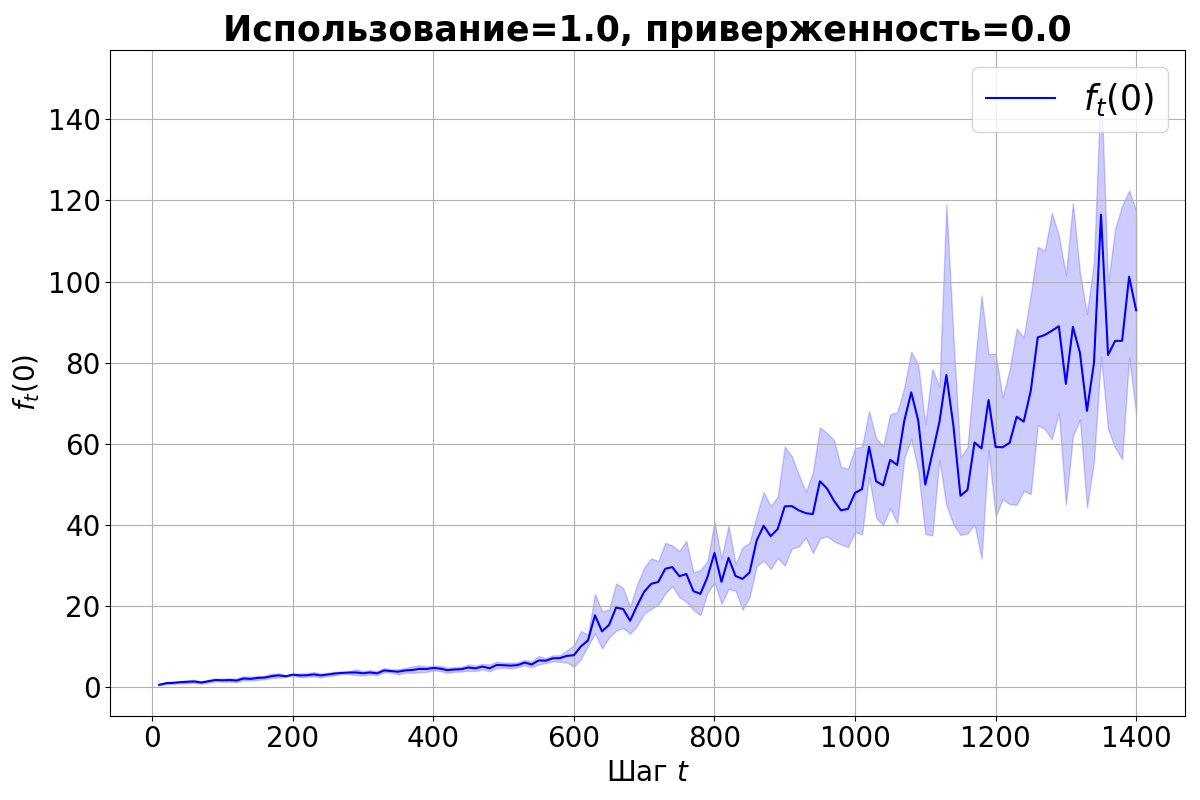
\includegraphics[width=0.32\linewidth]{pictures/ft0_sw_synthetic_sgd_model_50_1.0_0.0.png}~
        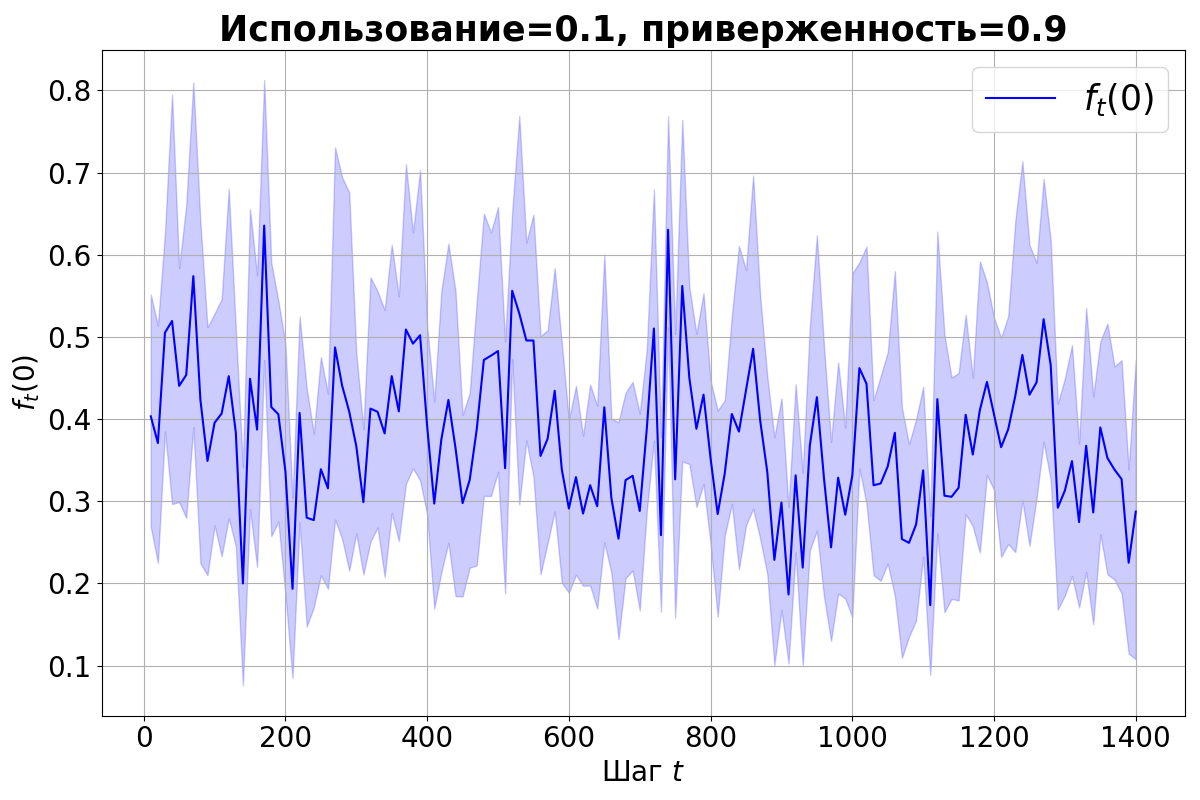
\includegraphics[width=0.32\linewidth]{pictures/ft0_sw_synthetic_sgd_model_50_0.1_0.9.png}~
        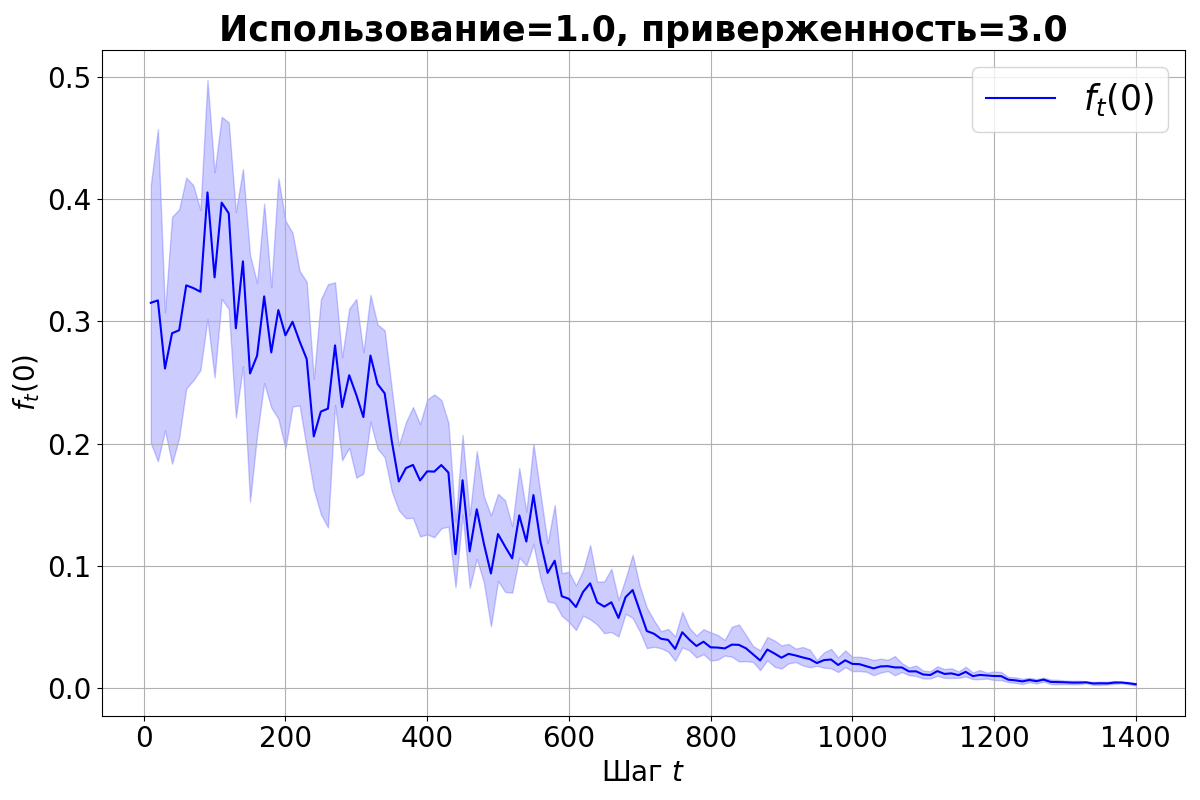
\includegraphics[width=0.32\linewidth]{pictures/ft0_sw_synthetic_sgd_model_50_1.0_3.0.png}

        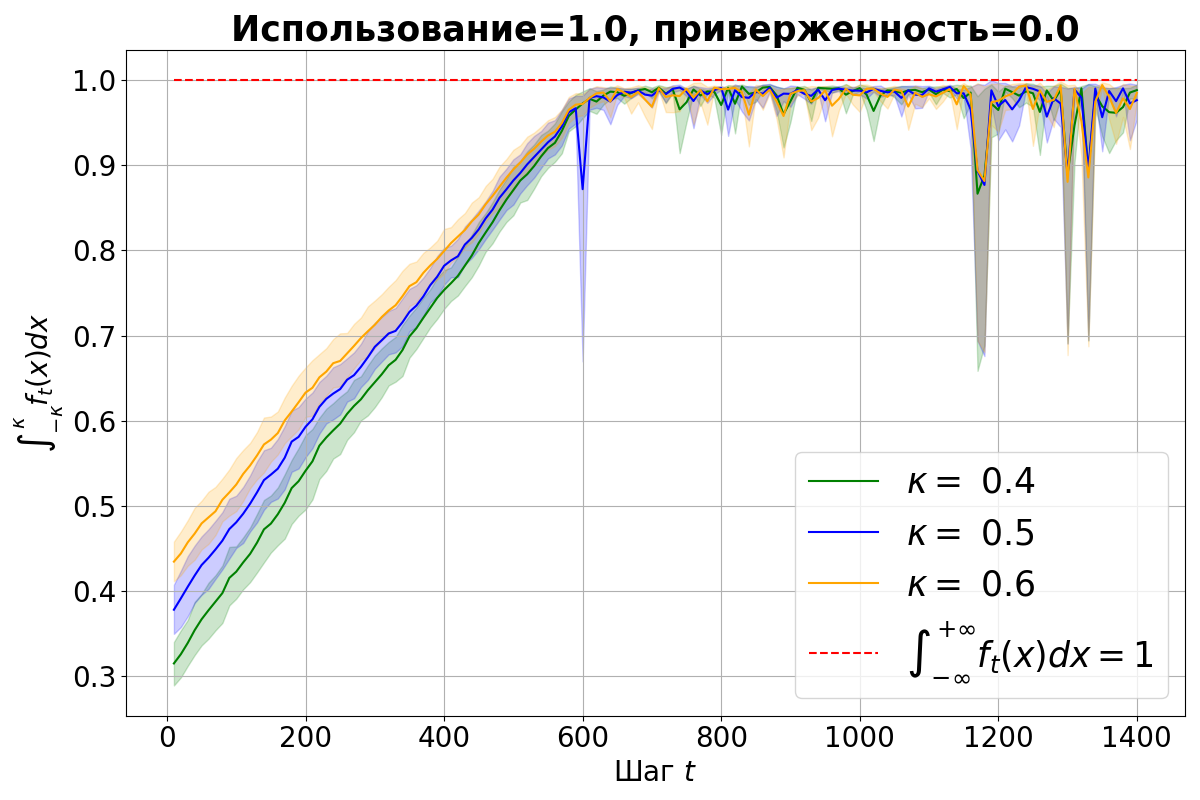
\includegraphics[width=0.32\linewidth]{pictures/int_sw_synthetic_sgd_model_50_1.0_0.0.png}~
        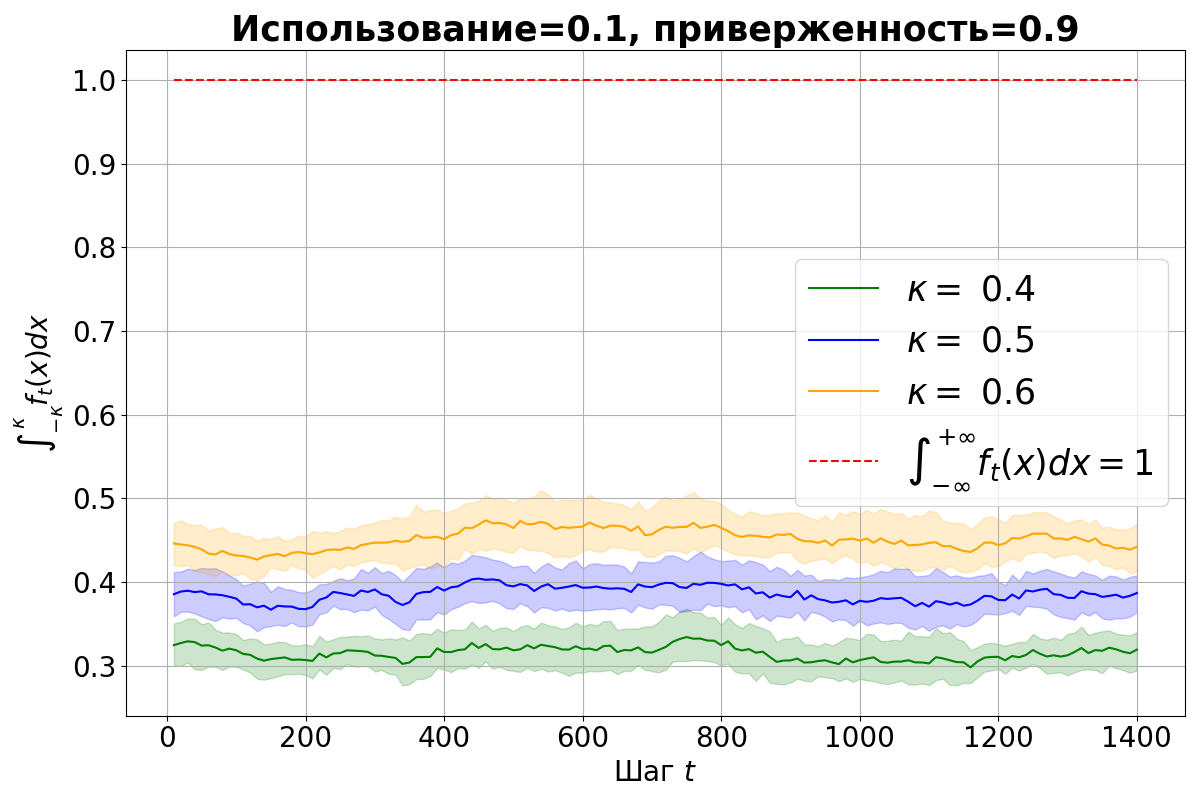
\includegraphics[width=0.32\linewidth]{pictures/int_sw_synthetic_sgd_model_50_0.1_0.9.png}~
        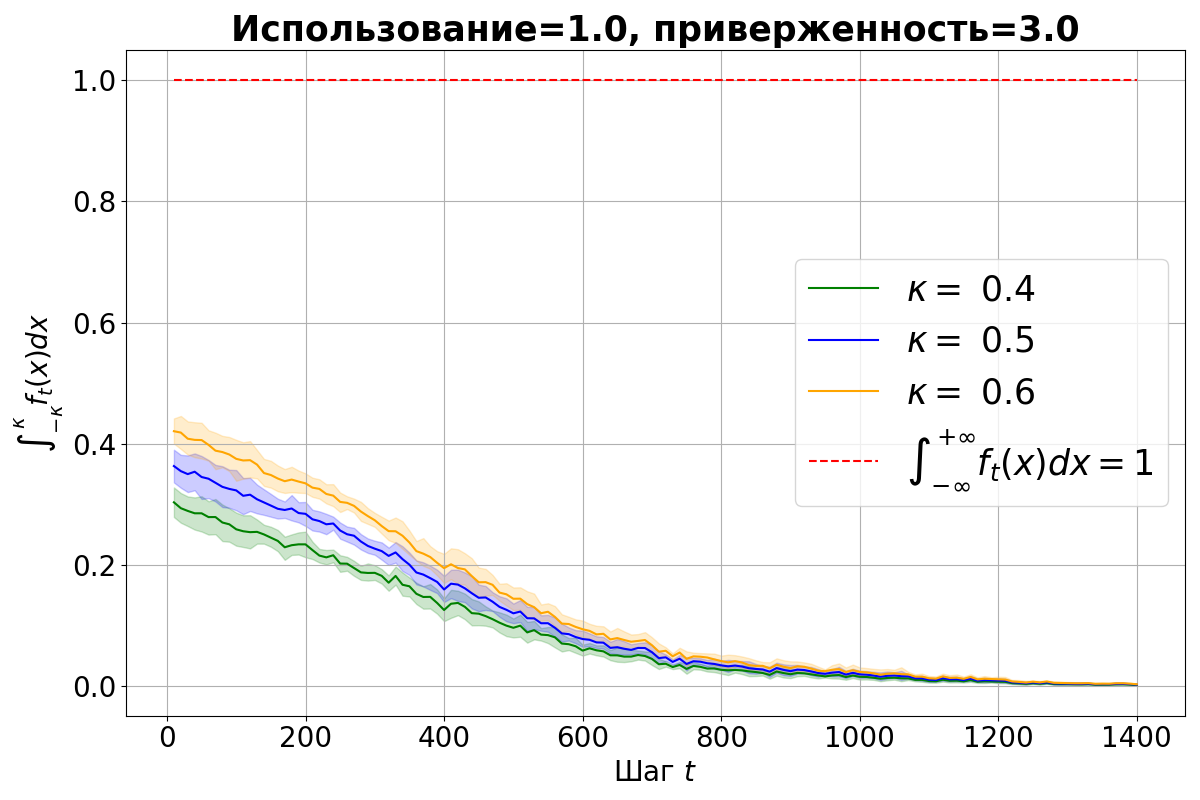
\includegraphics[width=0.32\linewidth]{pictures/int_sw_synthetic_sgd_model_50_1.0_3.0.png}
        
        \caption{Вычисление $f_t(0)$ и $\int_{-\kappa}^{\kappa}f_t(x)dx$ в постановке скользящее окно для линейной SGD модели на линейном наборе данных. Рассматриваются: использование, приверженность = $1$, $0$ (слева); $0,1$, $0,9$ (посередине); $1$, $3$ (справа). На этом рисунке виды все предельное множество системы \eqref{system} из Теоремы~\ref{delta}.}
        \label{delta_loop}
    \end{figure}

    \begin{figure}[h!]
        \centering
        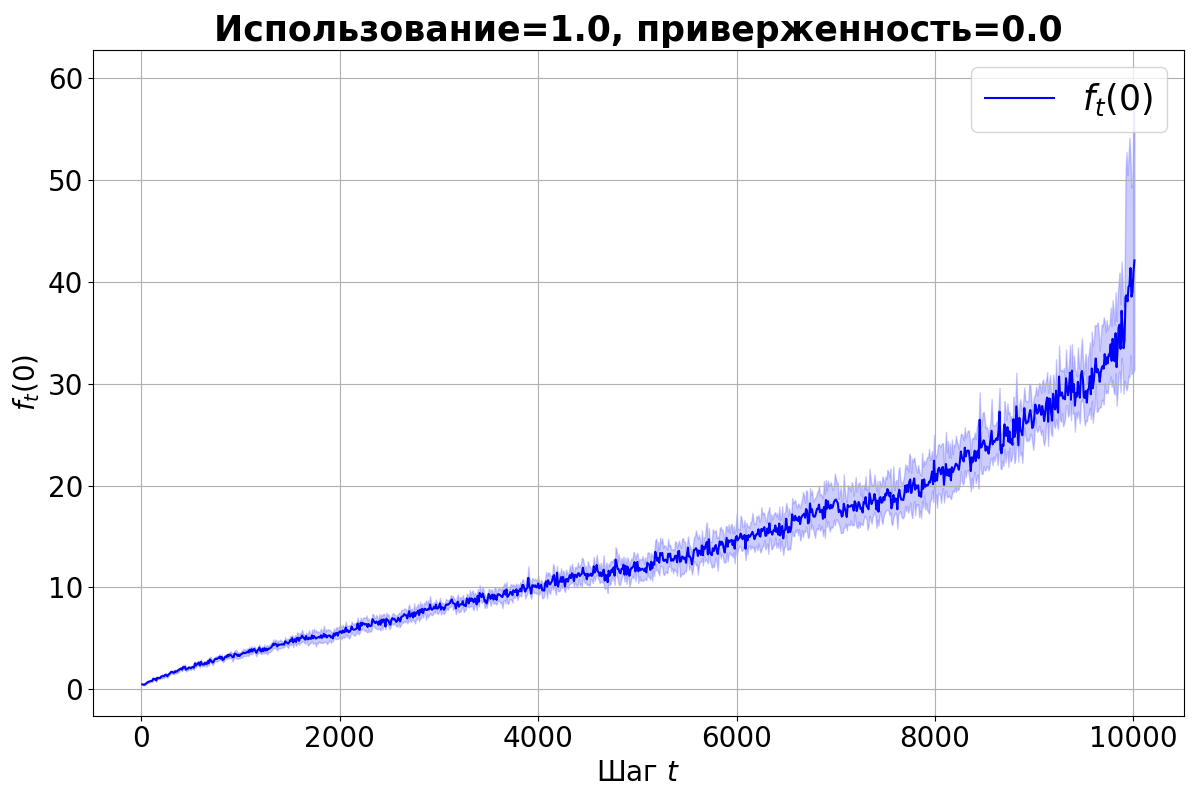
\includegraphics[width=0.32\linewidth]{pictures/ft0_su_synthetic_sgd_model_50_1.0_0.0.png}~
        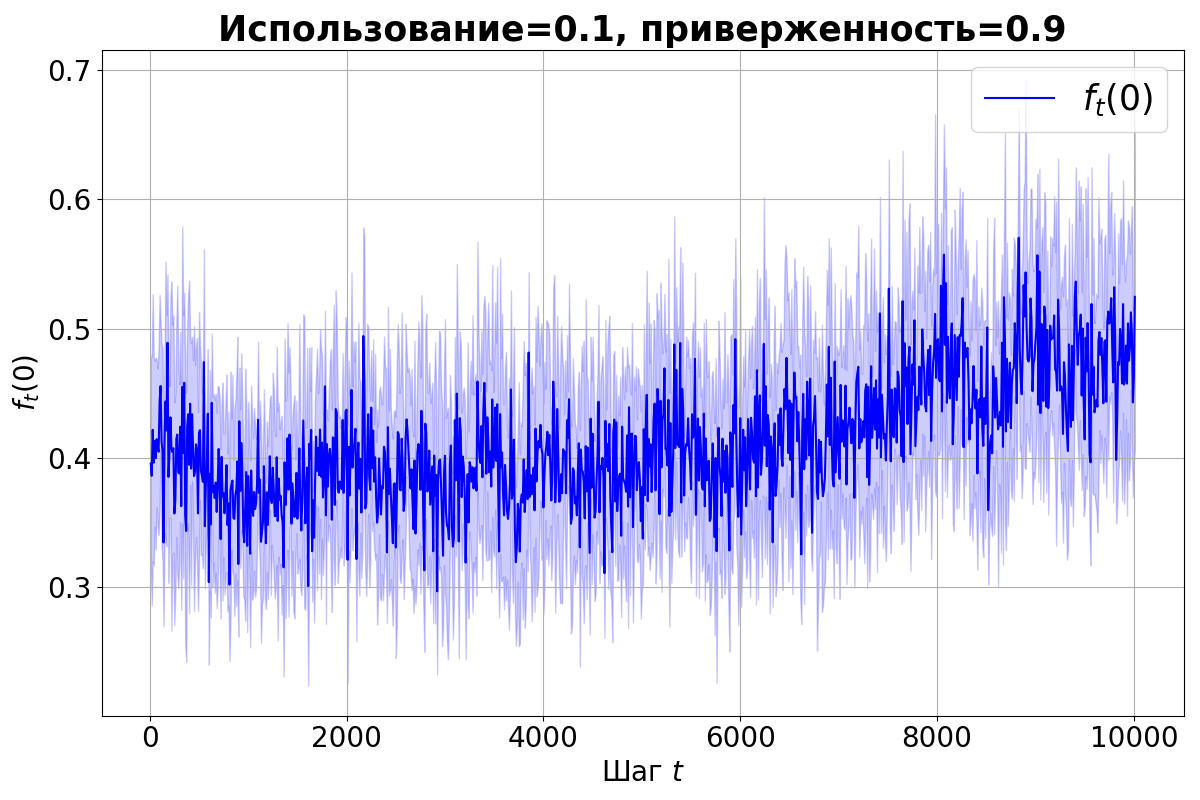
\includegraphics[width=0.32\linewidth]{pictures/ft0_su_synthetic_sgd_model_50_0.1_0.9.png}~
        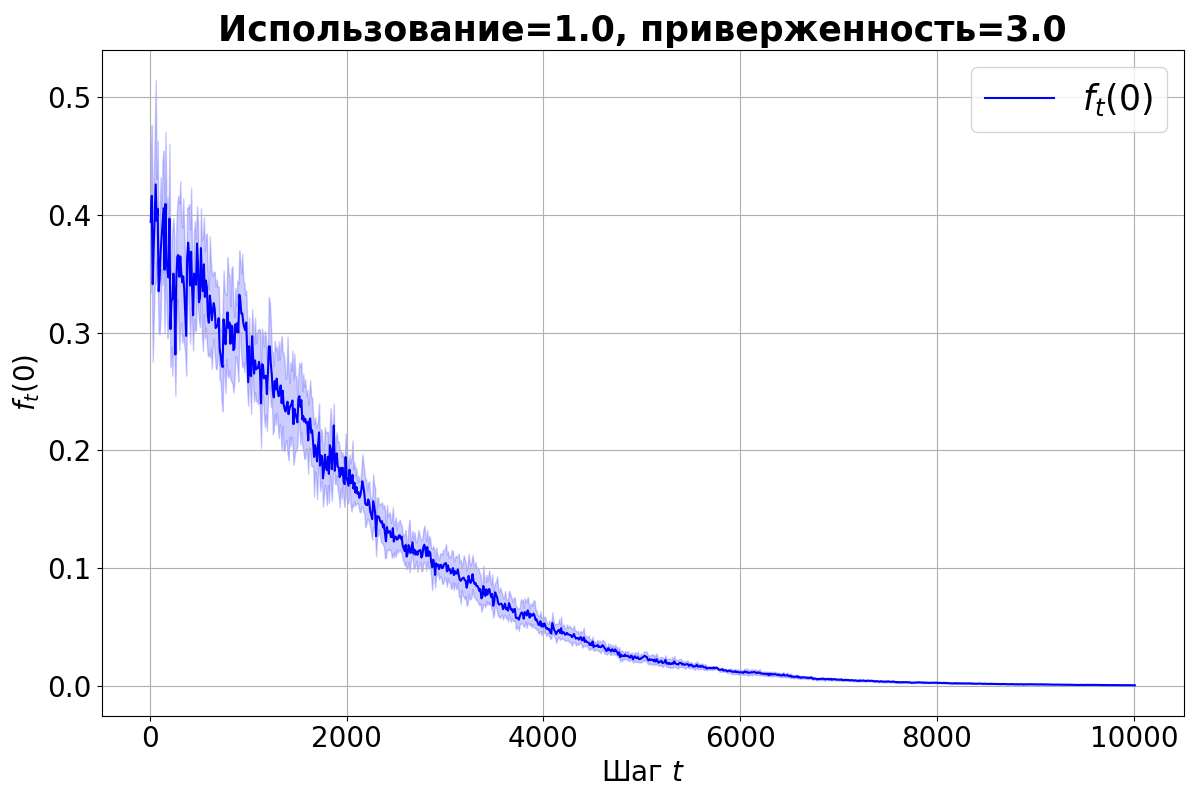
\includegraphics[width=0.32\linewidth]{pictures/ft0_su_synthetic_sgd_model_50_1.0_3.0.png}

        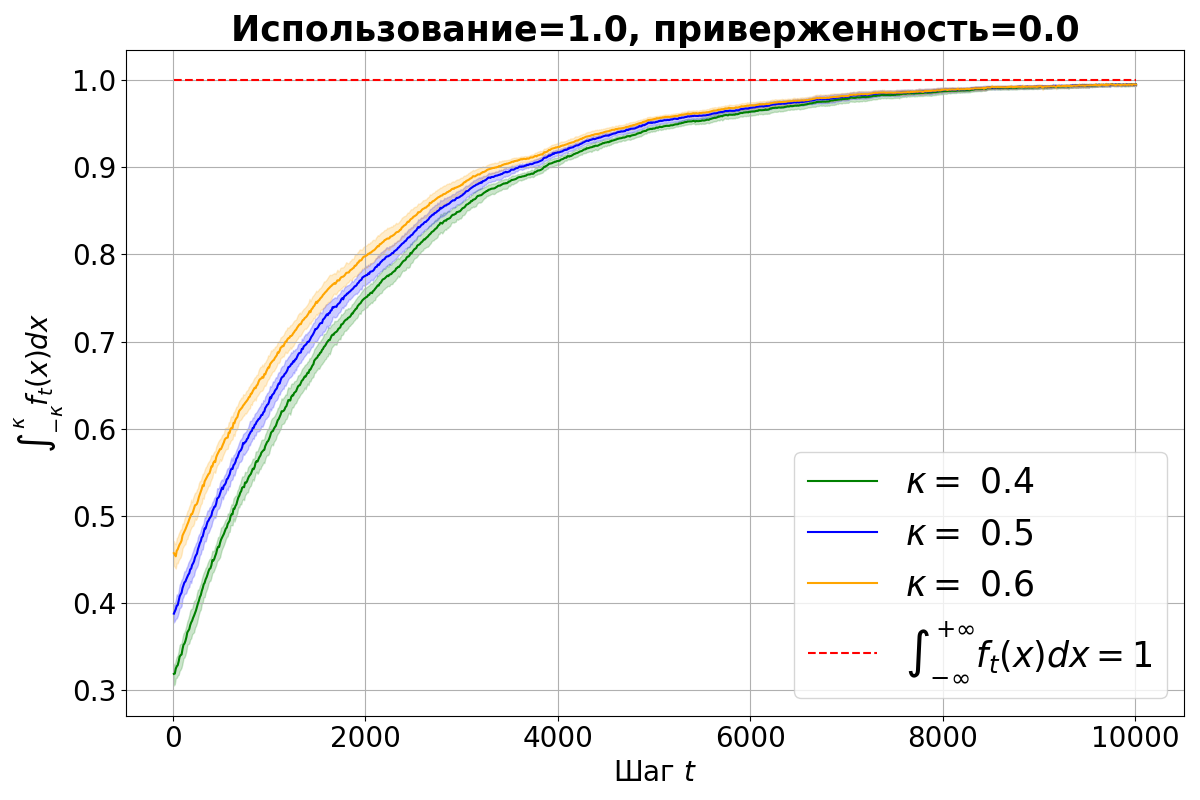
\includegraphics[width=0.32\linewidth]{pictures/int_su_synthetic_sgd_model_50_1.0_0.0.png}~
        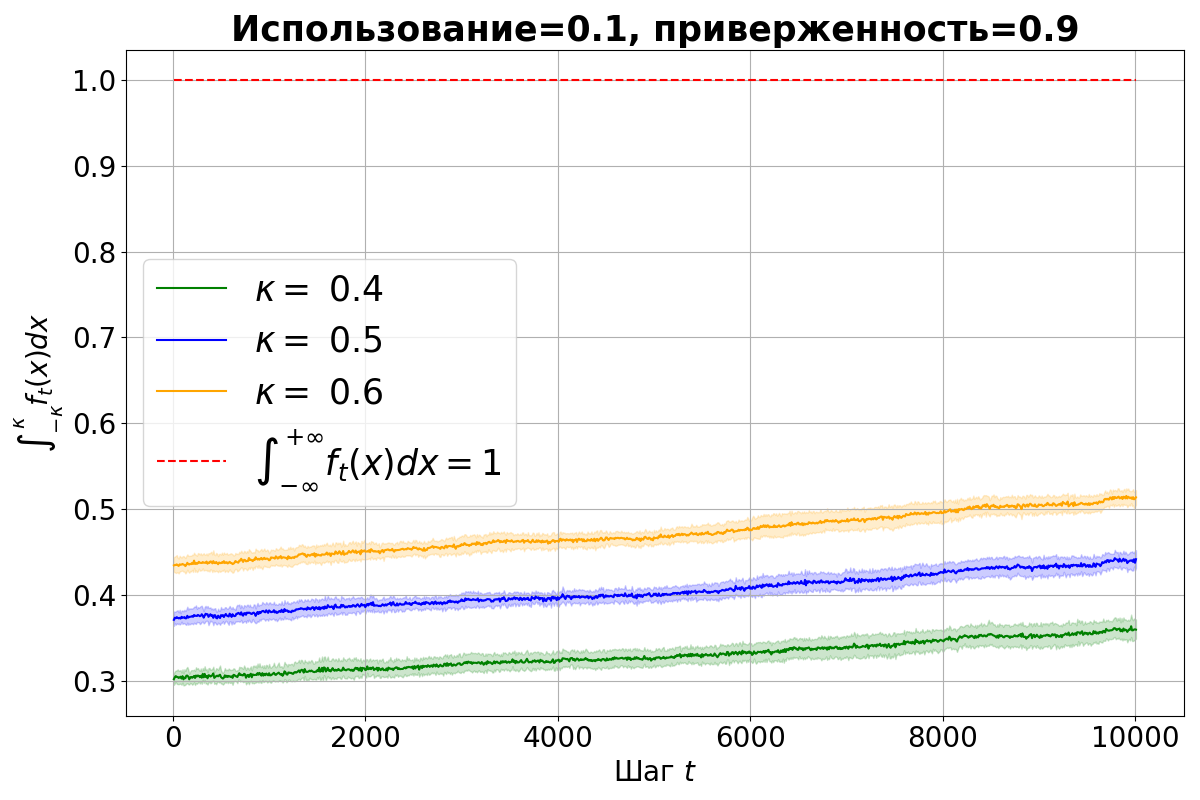
\includegraphics[width=0.32\linewidth]{pictures/int_su_synthetic_sgd_model_50_0.1_0.9.png}~
        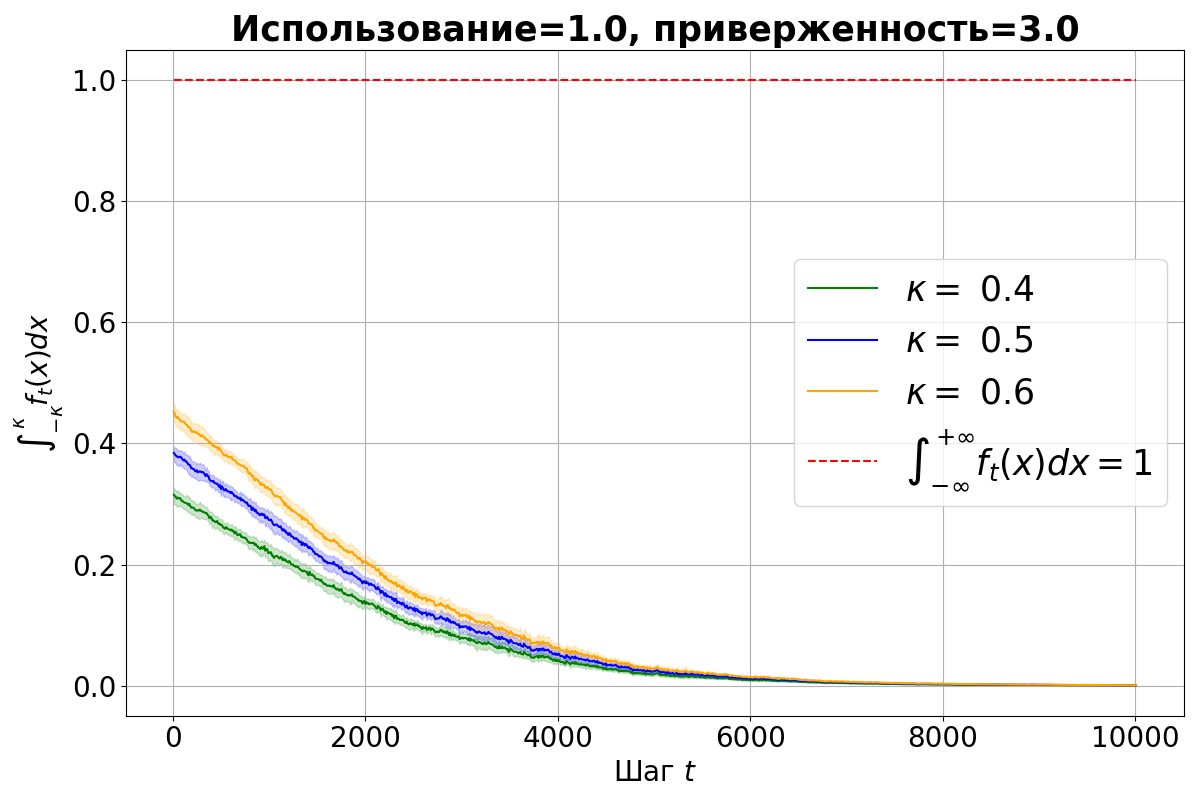
\includegraphics[width=0.32\linewidth]{pictures/int_su_synthetic_sgd_model_50_1.0_3.0.png}
        
        \caption{Вычисление $f_t(0)$ и $\int_{-\kappa}^{\kappa}f_t(x)dx$ в постановке обновление выборки для линейной SGD модели на линейном наборе данных. Рассматриваются: использование, приверженность = $1$, $0$ (слева); $0,1$, $0,9$ (посередине); $1$, $3$ (справа). На этом рисунке виды все предельное множество системы \eqref{system} из Теоремы~\ref{delta}.}
        \label{delta_sample}
    \end{figure}

    Как видно из этого эксперимента, при использовании $p = 1$ и приверженности $s = 3$ предельная плотность $\text{D}_{\overline{1, t}}(f_0)$, то есть плотность случайных векторов $y_i - y_i'$, есть нулевое распределение $\zeta(x)$. Это соответствует тому, что $\psi_t$ стремится к нулю и $\int_{-\kappa}^{\kappa}f_t(x)dx$ стремится к нулю.
    При использовании $p = 1$ и приверженности $s = 0$ наблюдается стремление к дельта-функции $\delta(x)$, то есть $\psi_t$ стремится к бесконечности, а $\int_{-\kappa}^{\kappa}f_t(x)dx$ стремится к единице. 
    Если использование $p = 0,1$ и приверженность $s = 0,9$, то плотность вероятности $y_i - y_i'$ остается почти такой же, то есть $\psi_t$ стремится к некоторой постоянной $c \in (0; +\infty)$. 

    Поэтому можно сделать вывод, что наблюдаемое поведение не противоречит утверждениям Теоремы~\ref{delta}.

    Дополнительные эксперименты для модели Ridge без регуляризации на наборе данных Фридмана приведены в Приложении~\ref{Appendix}. Поскольку форма этих графиков аналогична Рис.~\ref{delta_loop}~ и~\ref{delta_sample}, можно сделать вывод, что результаты Теоремы~\ref{delta} могут быть обобщены на различные наборы данных и модели машинного обучения.

\subsection{Проверка двух систем на автономность} \label{exp_4}

    В этом эксперименте проверяется утверждение \eqref{cond_semigroup} из Теоремы~\ref{semigroup}. Согласно обсуждению Теоремы~\ref{semigroup}, чтобы последовательность $\psi_t$ удовлетворяла условию \eqref{cond_semigroup}, она должна быть степенной последовательностью.

    В этом эксперименте тестируется автономность систем скользящего окна и обновления выборки. Первая система не является автономной, а вторая является автономной по конструкции, поскольку оператор эволюции $\text{D}_t$, то есть алгоритм обучения и процедура обратной связи, не зависит от шага по времени, $\text{D}_t = \text{D}$.
    Для проверки автономность строится график $\ln(f_t(0))$ и проверяется, есть ли прямая линия, когда система автономна, или нет прямой линии для не автономной системы. Для наглядности строится линейную модель измерений и измеряется $r^2$-score -- статистическую меру того, насколько хорошо прямая соответствует данным. Наблюдения показаны на Рис.~\ref{fig_exp_4_1}-\ref{fig_exp_4_4}. В эксперименте использовались линейная SGD модель и RidgeCV на линейном наборе данных и наборе данных Фридмана.

    \begin{figure}[h!]
        \centering
        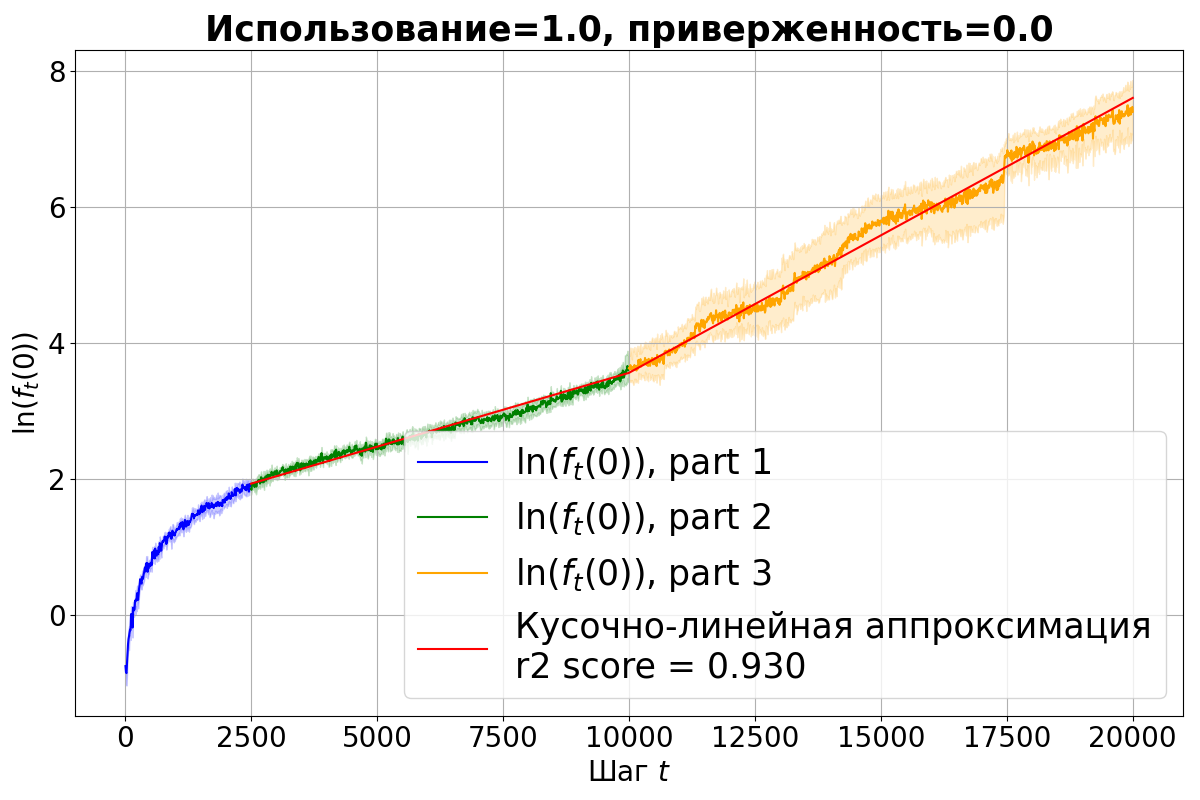
\includegraphics[width=0.32\linewidth]{pictures/aut_su_synthetic_sgd_model_50_1.0_0.0.png}
        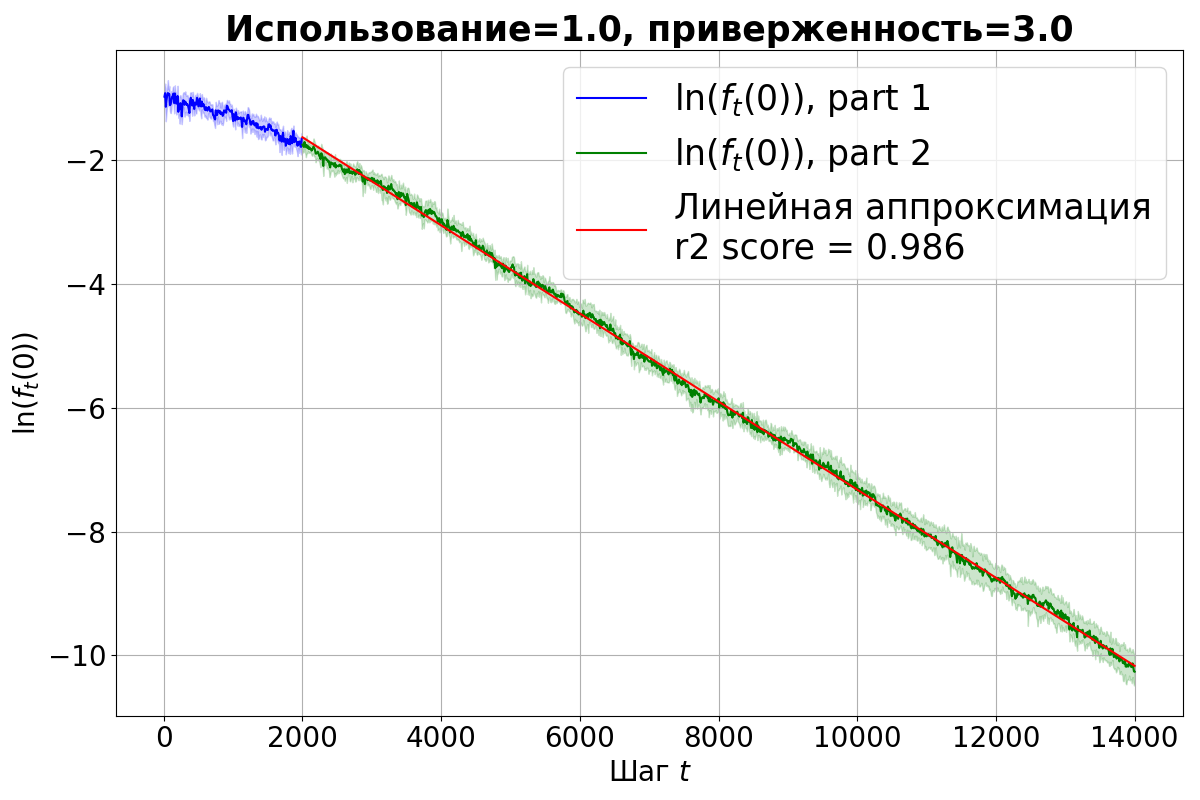
\includegraphics[width=0.32\linewidth]{pictures/aut_su_synthetic_sgd_model_50_1.0_3.0.png}
        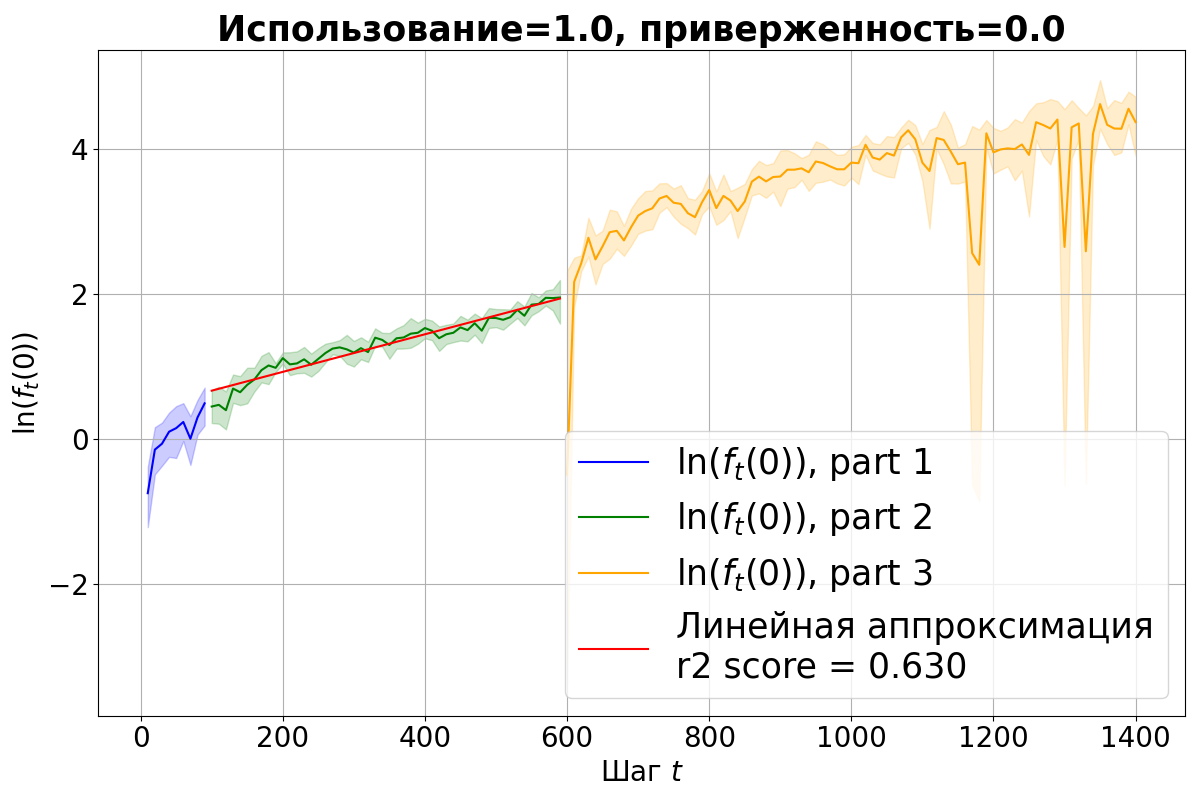
\includegraphics[width=0.32\linewidth]{pictures/aut_sw_synthetic_sgd_model_50_1.0_0.0.png}
        
        \caption{Проверка двух систем на автономность. Обновление выборки (слева и посередине) и скользящее окно (справа). Результаты для линейной SGD модели на синтетическом линейном наборе данных.}
        \label{fig_exp_4_1}
    \end{figure}

    \begin{figure}[h!]
        \centering
        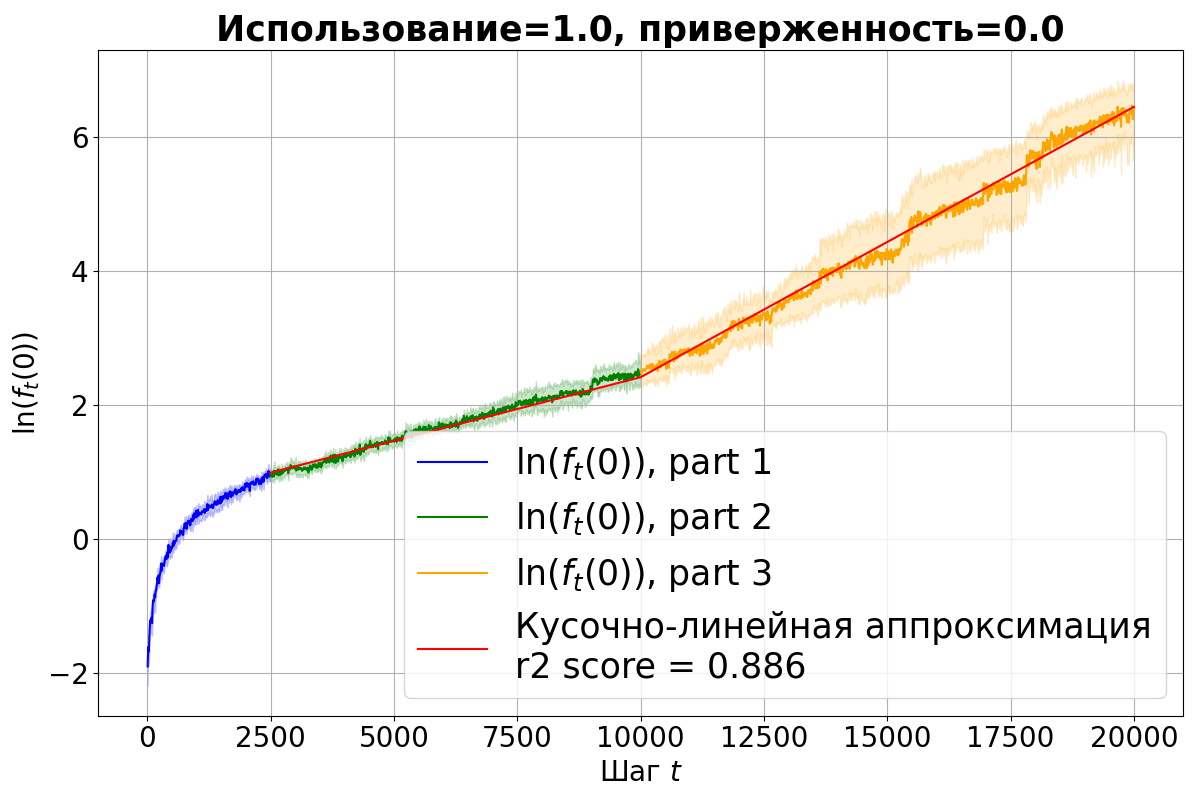
\includegraphics[width=0.32\linewidth]{pictures/aut_su_friedman_sgd_model_50_1.0_0.0.png}
        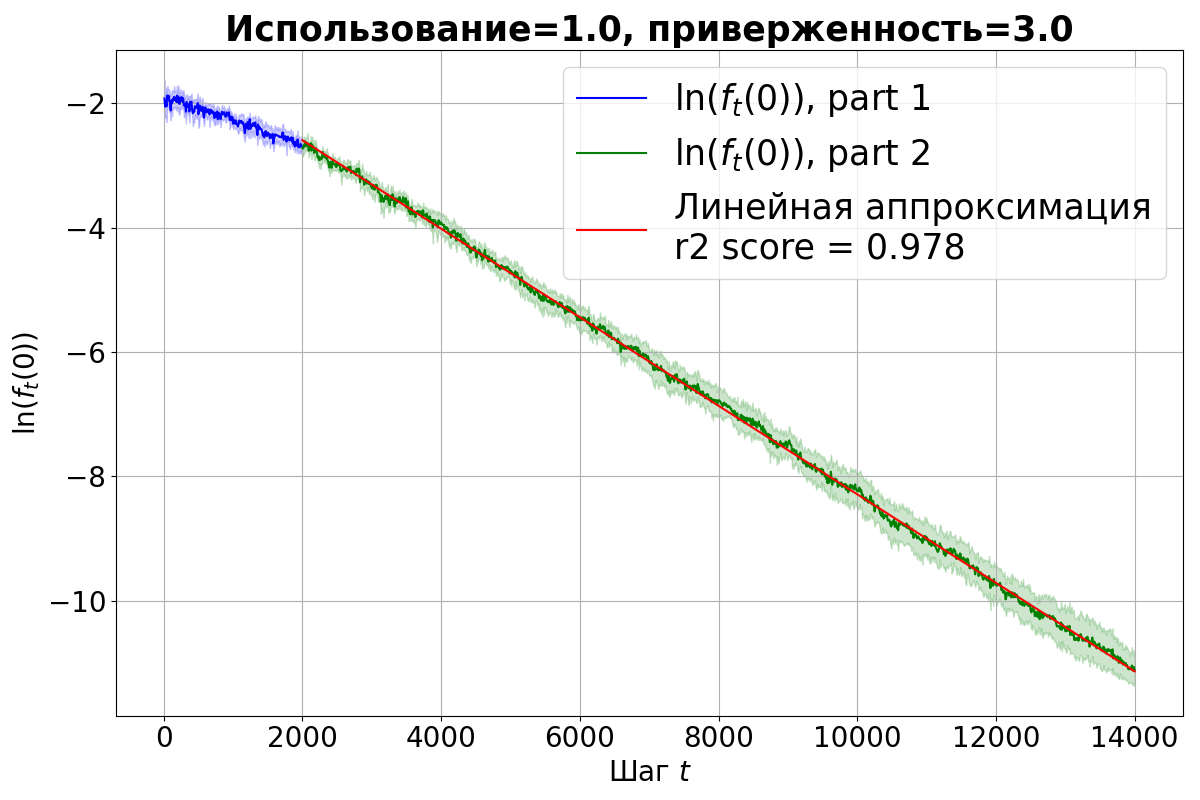
\includegraphics[width=0.32\linewidth]{pictures/aut_su_friedman_sgd_model_50_1.0_3.0.png}
        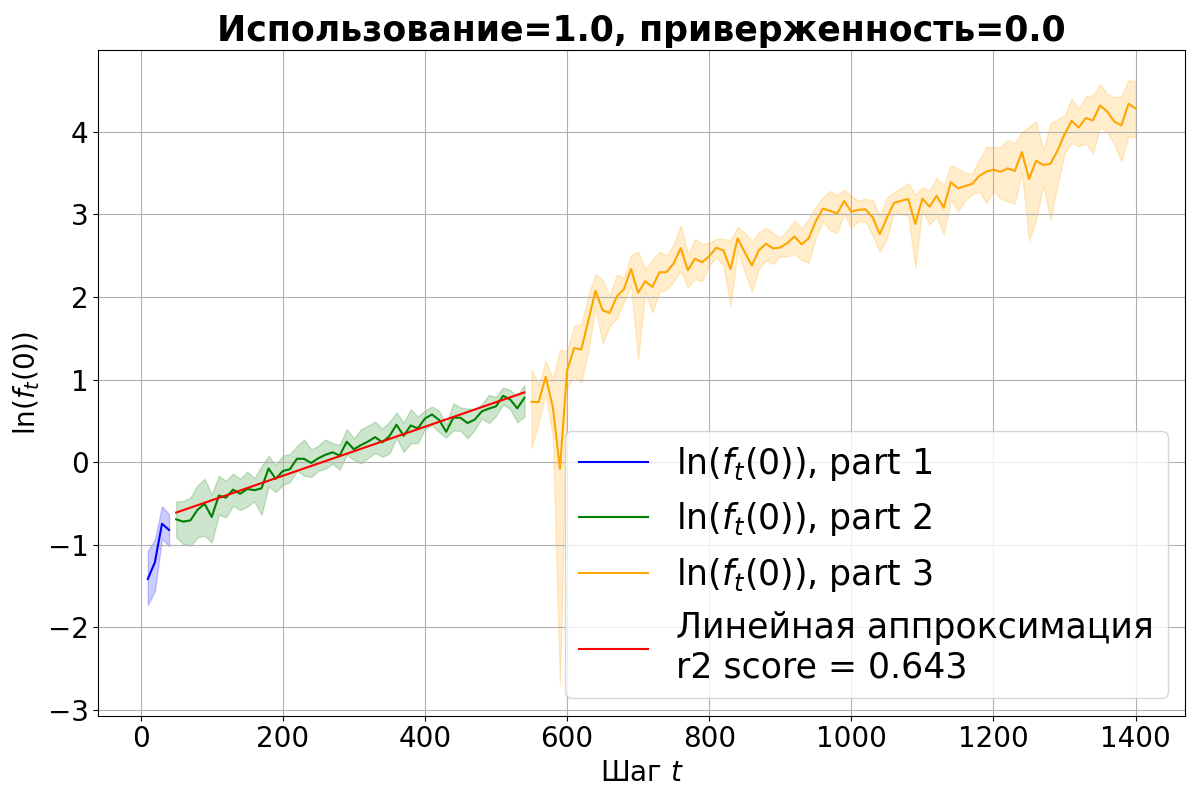
\includegraphics[width=0.32\linewidth]{pictures/aut_sw_friedman_sgd_model_50_1.0_0.0.png}
        
        \caption{Проверка двух систем на автономность. Обновление выборки (слева и посередине) и скользящее окно (справа). Результаты для линейной SGD модели на датасета Фридмана.}
        \label{fig_exp_4_2}
    \end{figure}

    \begin{figure}[h!]
        \centering
        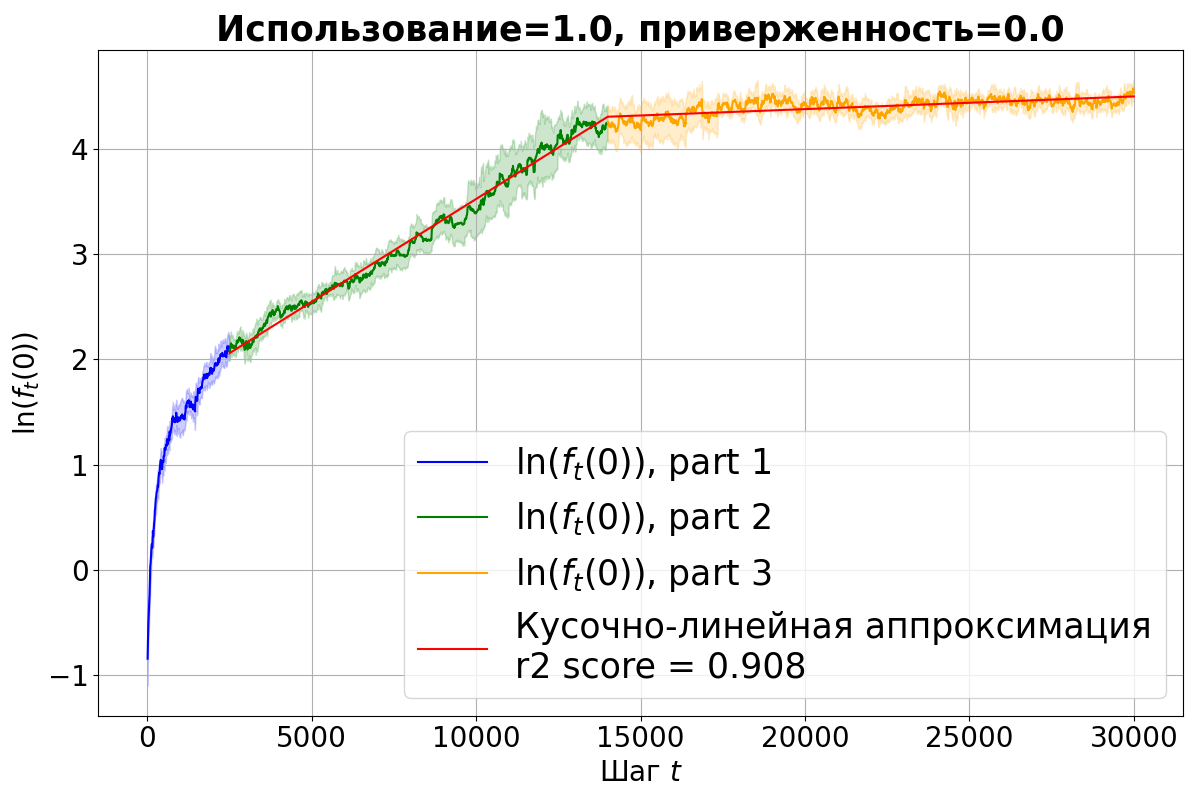
\includegraphics[width=0.32\linewidth]{pictures/aut_su_synthetic_ridgecv_model_1.0_0.0.png}
        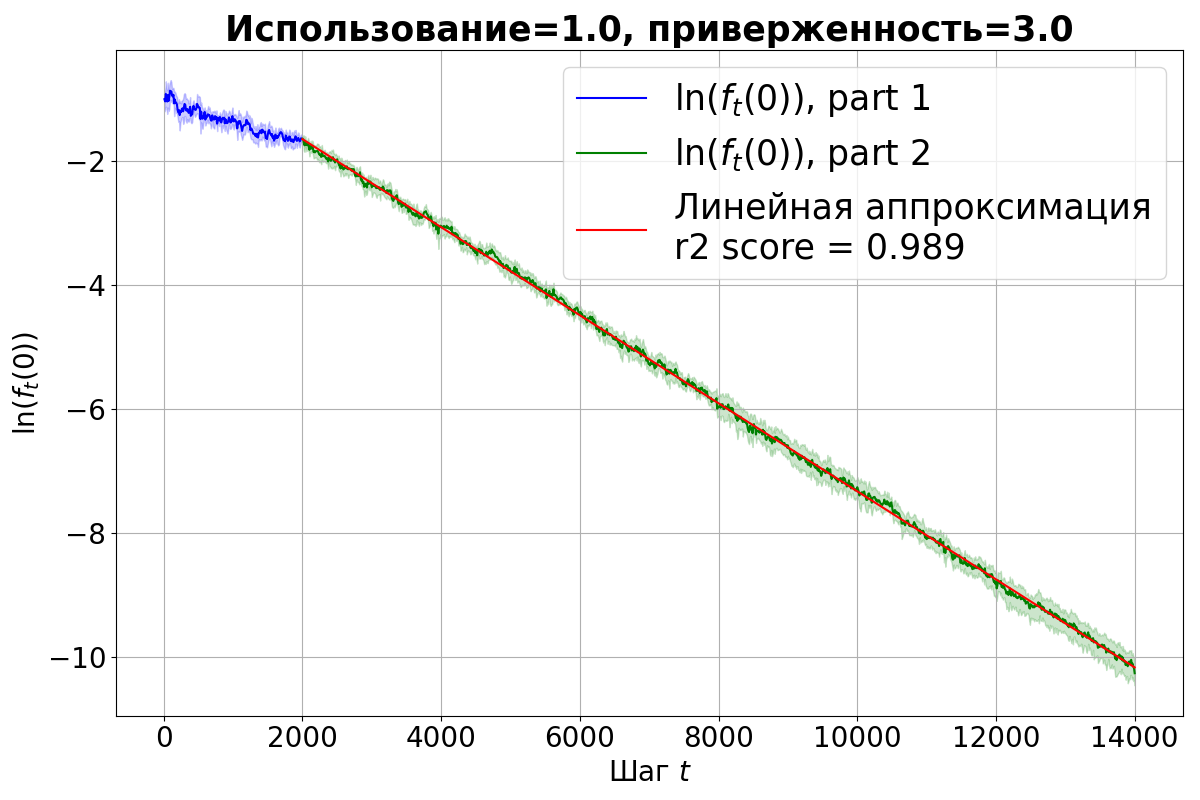
\includegraphics[width=0.32\linewidth]{pictures/aut_su_synthetic_ridgecv_model_1.0_3.0.png}
        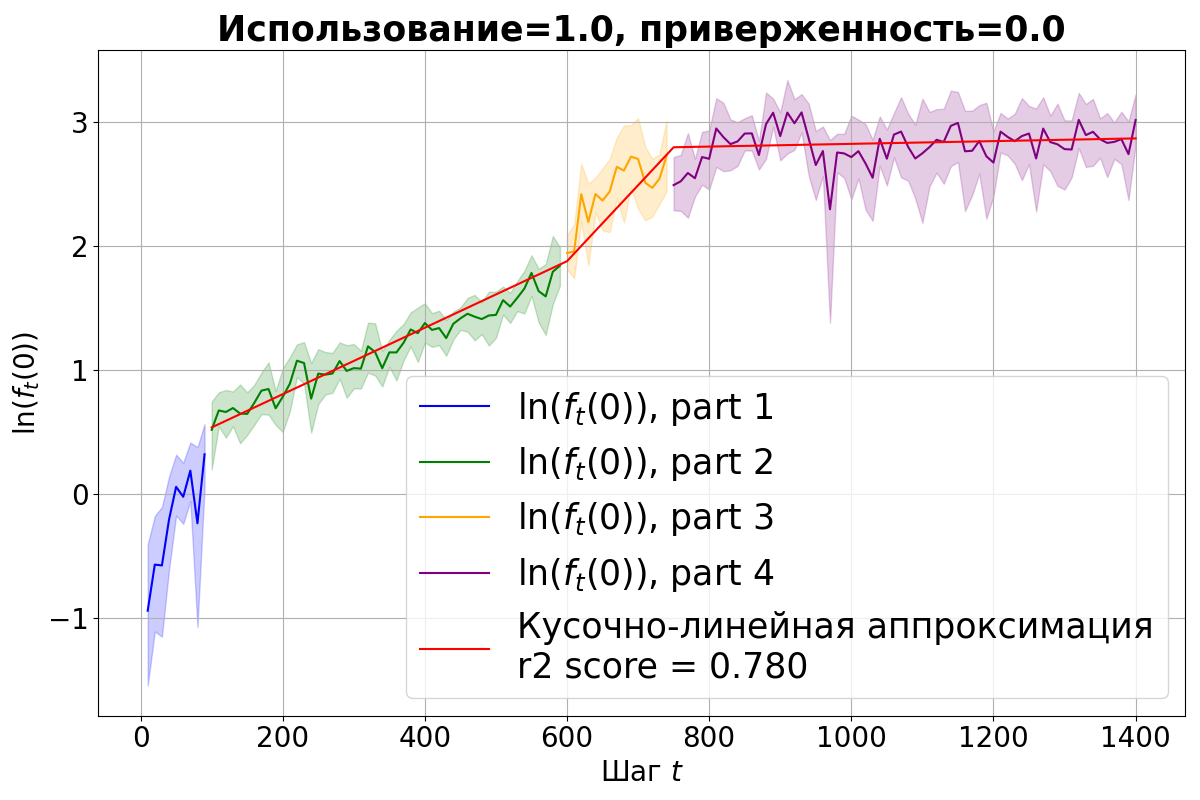
\includegraphics[width=0.32\linewidth]{pictures/aut_sw_synthetic_ridgecv_model_1.0_0.0.png}
        
        \caption{Проверка двух систем на автономность. Обновление выборки (слева и посередине) и скользящее окно (справа). Результаты для модели RidgeCV на синтетическом линейном наборе данных.}
        \label{fig_exp_4_3}
    \end{figure}

    \begin{figure}[h!]
        \centering
        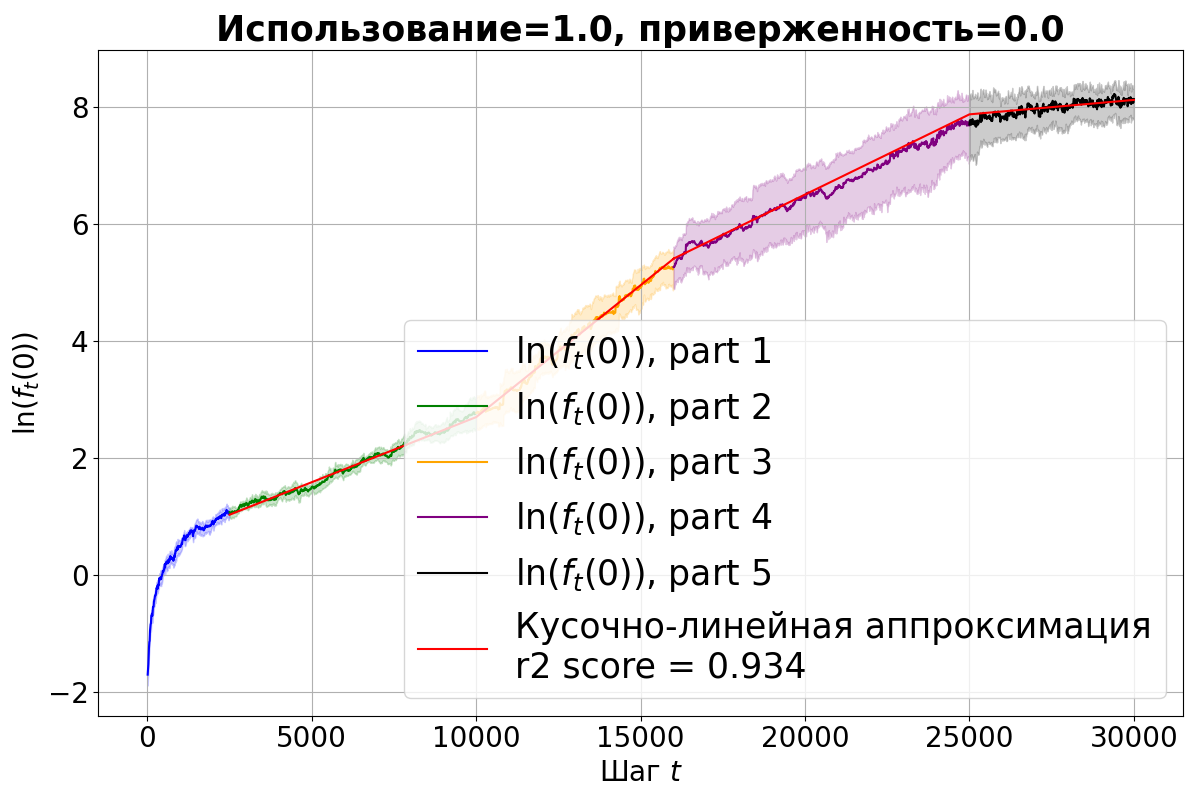
\includegraphics[width=0.32\linewidth]{pictures/aut_su_friedman_ridgecv_model_1.0_0.0.png}
        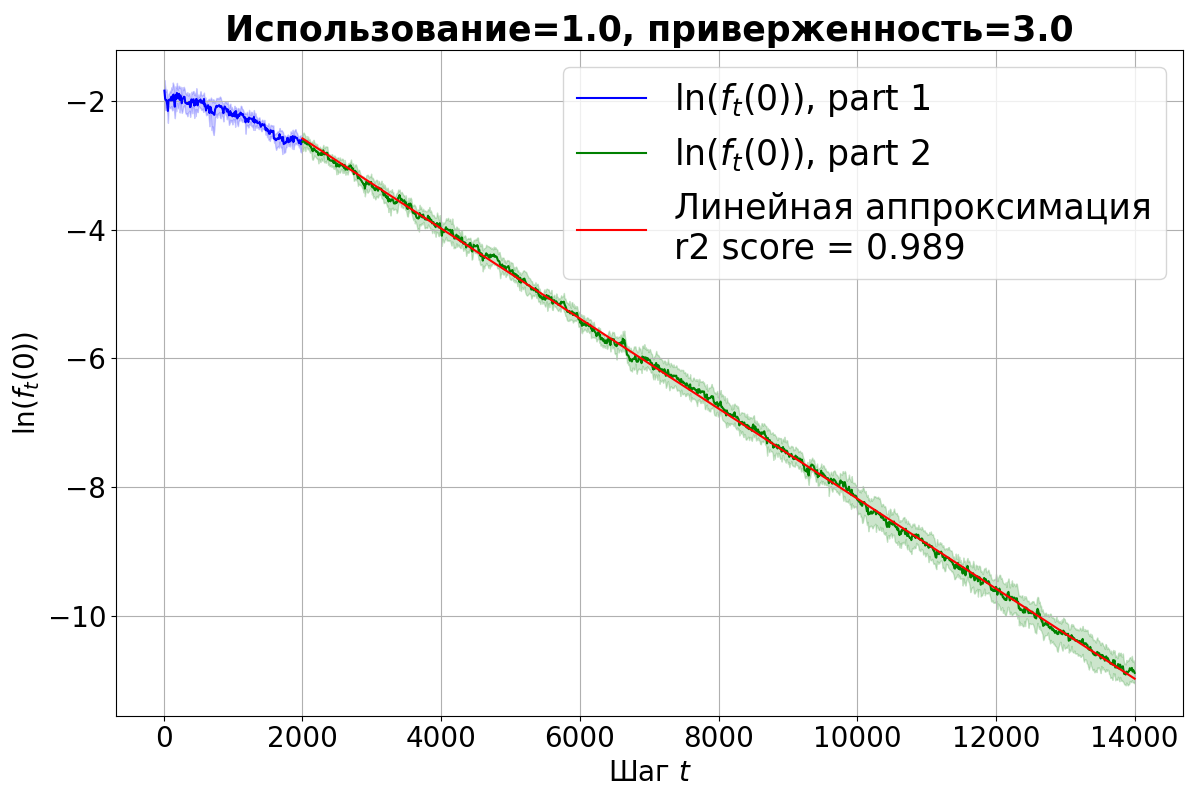
\includegraphics[width=0.32\linewidth]{pictures/aut_su_friedman_ridgecv_model_1.0_3.0.png}
        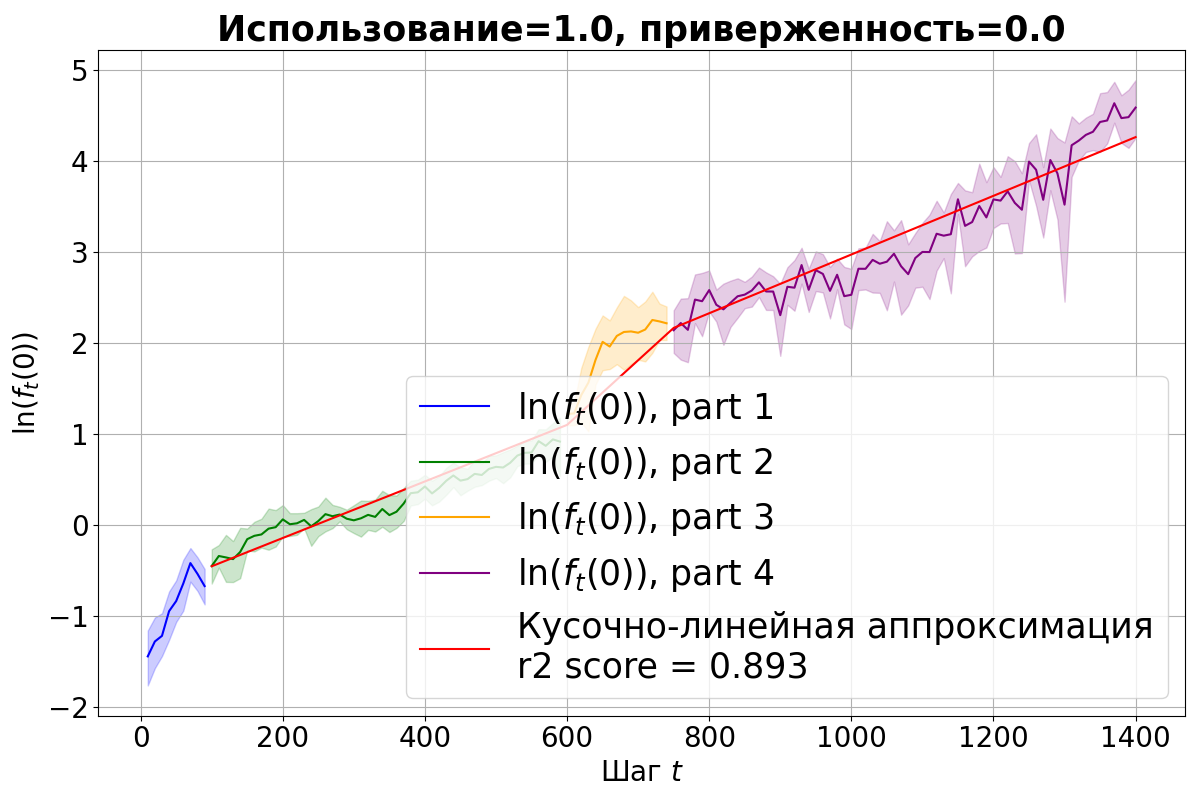
\includegraphics[width=0.32\linewidth]{pictures/aut_sw_friedman_ridgecv_model_1.0_0.0.png}
        
        \caption{Проверка двух систем на автономность. Обновление выборки (слева и посередине) и скользящее окно (справа). Результаты для модели RidgeCV на наборе данных Фридмана.}
        \label{fig_exp_4_4}
    \end{figure}

    Как видно из результатов эксперимента, в случае постановки скользящее окно линейная аппроксимация плохо приближает данные, поэтому эта система не является автономной. На графиках заметно изменение в районе $t = 600$, это соответствует точке, где доля повторно используемых предсказаний в данных стабилизируется при использовании $p$ и далее не меняется. Постановка обновления выборки в случае использования $p = 1$ и приверженности $s = 3$ является автономной для всех моделей и наборов данных, поскольку наблюдается хорошее линейное приближение. В случае использования $p = 1$ и приверженности $s = 0$ наблюдаются два линейных сегмента, за исключением случая RidgeCV на наборе данных Фридмана. Хотя наша гипотеза утверждает, что должен быть только один линейный сегмент, видны две области автономности. Это может быть связано с тем, что при $t \approx 10000$ все элементы исходного набора данных заменяются предсказаниями модели.

    Для приближения данных прямой линией используется робастный регрессор Хубера. Мы также проводим тест Бреуша-Пагана-Лагранжа на гомоскедастичность \citep{d1971omnibus}. В постановке обновление выборки получаются $p$-value $\approx 10^{-18}$, а в постановке скользящее окно $p$-value равно $0,001$. Таким образом остатки во всех случаях гомоскедастичны и линейная аппроксимация оправдана.

    Из этого можно сделать вывод, что утверждения Теоремы~\ref{semigroup} не противоречат наблюдениям в данном эксперименте. Гипотезы об автономности двух систем частично подтвердились.

\subsection{Стремление моментов к нулю} \label{exp_5}

    В этом эксперименте сравниваются предсказания Леммы~\ref{moments} с наблюдениями. В постановке скользящее окно проверяется третье утверждение этой Леммы: $\|\{\nu_k^t\}_{k=1}^{\infty}\|_1 = \sum_{k=1}^{+\infty} |\nu_k^t| \underset{t \to +\infty}{\longrightarrow} 0$. По соображениям вычислительной эффективности мы сообщаем только $\sum_{k=1}^{N} |\nu_k^t|$ для $N=300$.

    В постановке обновление выборки проверяется второе утверждение Леммы, то есть $\nu_k^t \underset{t \to +\infty}{\longrightarrow} 0$ для $k = 1, 2, ... , 6$. Наблюдения для этого эксперимента показаны на Рис.~\ref{fig_exp_5_1}~и~\ref{fig_exp_5_2}. Все результаты в этом эксперименте получены для линейной SGD модели на линейном наборе данных и наборе данных Фридмана.

    \begin{figure}[h!]
        \centering
        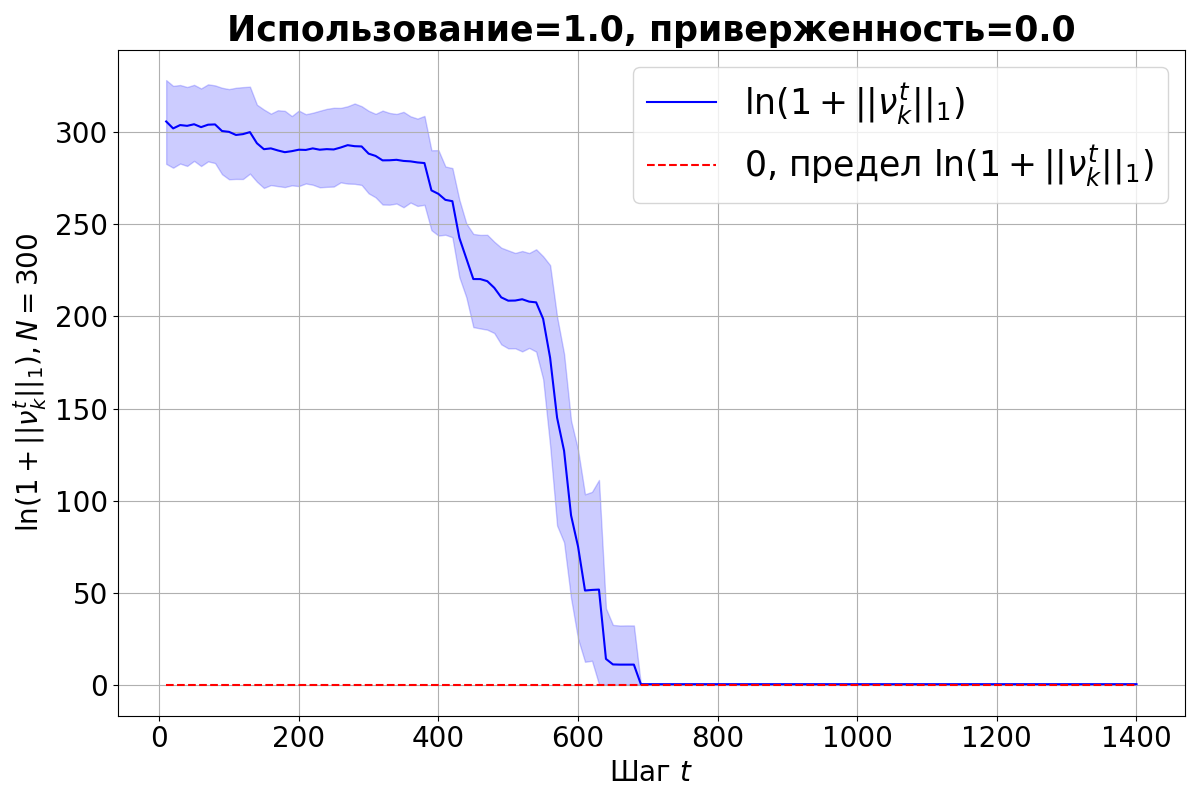
\includegraphics[width=0.49\linewidth]{pictures/k_mom_sw_synthetic_sgd_model_50_1.0_0.0.png}
        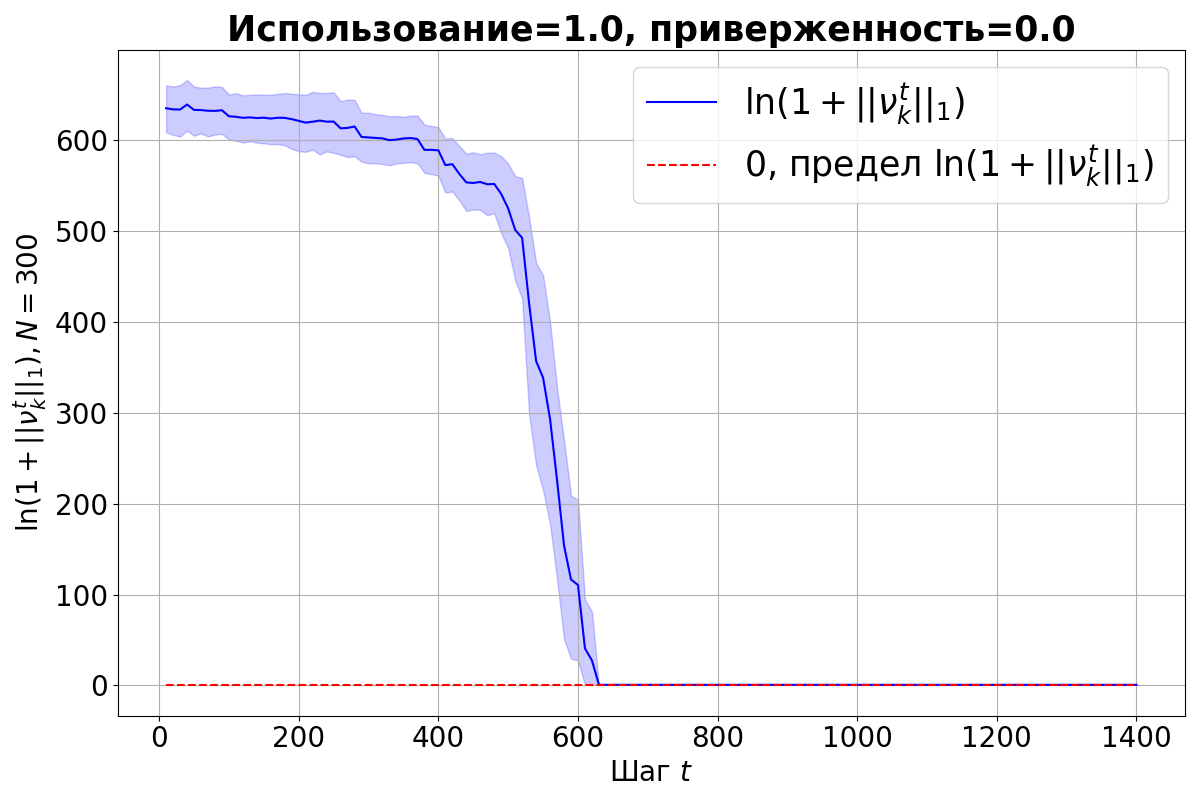
\includegraphics[width=0.49\linewidth]{pictures/k_mom_sw_friedman_sgd_model_50_1.0_0.0.png}
        
        \caption{Измерение $\|\{\nu_k^t\}_{k=1}^{\infty}\|_1$ в постановке скользящее окно. Линейный набор данных (слева) и набор данных Фридмана (справа). Как можно видеть, третье утверждение Леммы~\ref{moments} выполняется.}
        \label{fig_exp_5_1}
    \end{figure}

    \begin{figure}[h!]
        \centering
        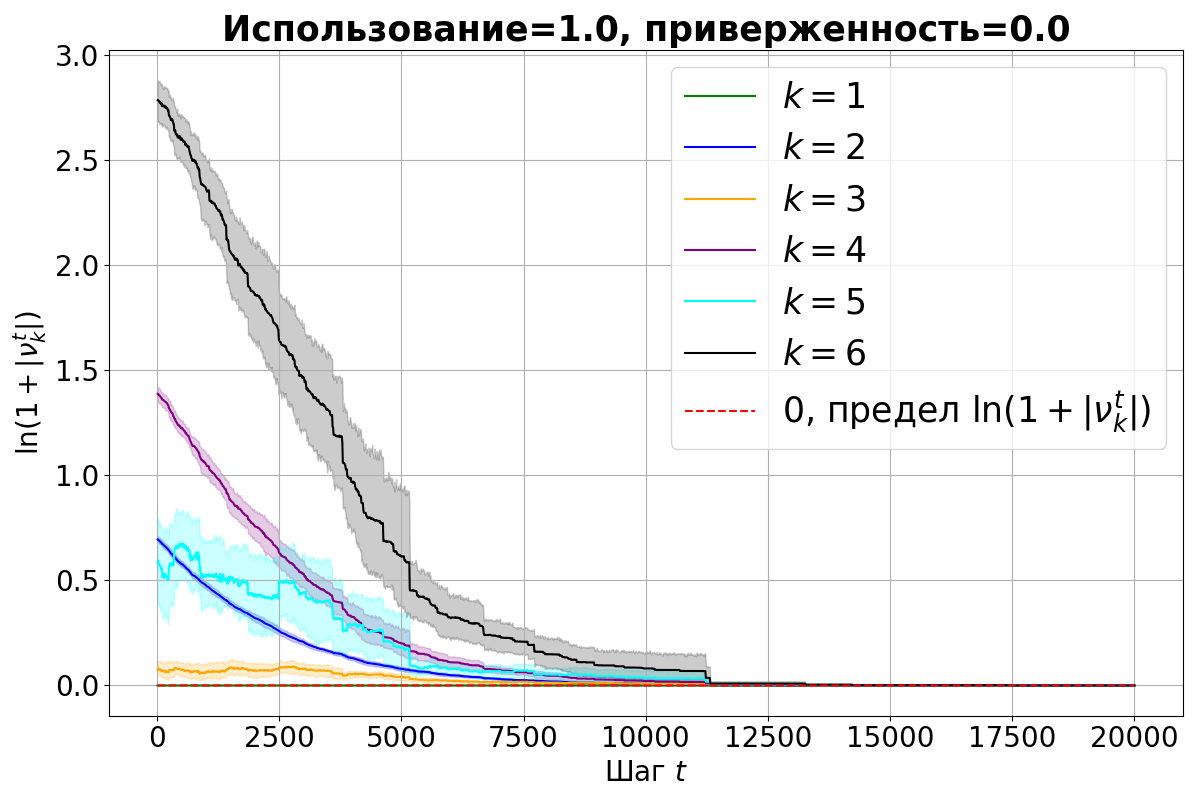
\includegraphics[width=0.49\linewidth]{pictures/k_mom_su_synthetic_sgd_model_50_1.0_0.0.png}
        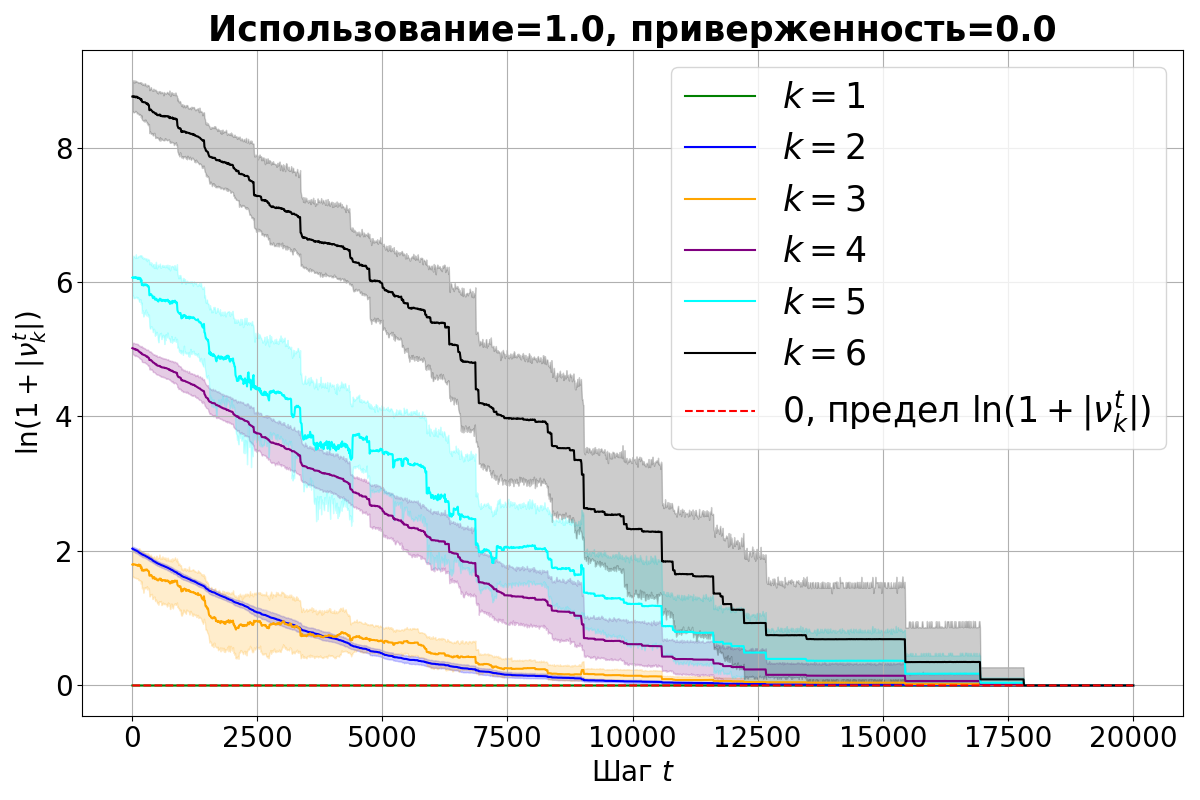
\includegraphics[width=0.49\linewidth]{pictures/k_mom_su_friedman_sgd_model_50_1.0_0.0.png}
        
        \caption{Измерение $\nu_k^t$ для $k = 1, 2, ... , 6$ для постановки обновление выборки. Линейный набор данных (слева) и набор данных Фридмана (справа). Как можно видеть, второе утверждение Леммы~\ref{moments} выполняется.}
        \label{fig_exp_5_2}
    \end{figure}

    \newpage

    Как видно из результатов эксперимента, второе и третье утверждения Леммы~\ref{moments} выполняются во всех случаях. При использовании $p = 1$ и приверженности $s = 0$ пределом плотности распределений $y_i - y_i'$, является дельта-функция $\delta(x)$. Однако в экспериментах не наблюдается в точности ноль, как показывает график, поскольку во всех случаях рассматривается только конечные значения $t$.


    

    






    



